\documentclass[10pt, a4paper]{article}
\usepackage[left=2.00cm, right=2.00cm, top=2.00cm, bottom=2.00cm]{geometry}
\usepackage{supertabular}
\usepackage{graphicx}
\usepackage{float}
\usepackage[fontset=windows]{ctex}
\usepackage{amsmath,amssymb,amsthm}
\usepackage{unicode-math}
\usepackage{verbatim}
\usepackage{multirow}
\usepackage{pifont}
\usepackage{caption}
\usepackage{diagbox}
\usepackage{listings}
\usepackage{algorithm}  
\usepackage{algpseudocode}
\usepackage{booktabs}   
\usepackage{underscore}
\usepackage{xcolor}
\lstset{
  %行号
  numbers=left,
  %背景框
  frame=single,
  rulecolor=\color[rgb]{0.8,0.8,0.8},         % 设置代码框颜色
  breaklines,                                 % 自动将长的代码行换行排版
  extendedchars=false,                        % 解决代码跨页时,章节标题,页眉等汉字不显示的问题
  %背景色
  %backgroundcolor=\color[rgb]{1,1,0.76},
  backgroundcolor=\color[RGB]{245,245,244},
  %样式
  keywordstyle=\bf\color{blue},
  identifierstyle=\bf,
  numberstyle=\color[RGB]{0,192,192},
  commentstyle=\it\color[RGB]{0,96,96},
  stringstyle=\rmfamily\slshape\color[RGB]{128,0,0},
  %显示空格
  showstringspaces=false
}
% \begin{figure}[H]
%     \centering
%     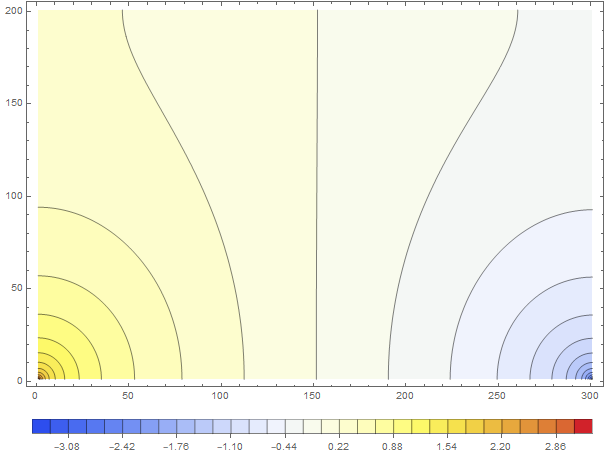
\includegraphics[width=0.4\textwidth]{Q1(1).png}
%     \caption{Q1(1)}\label{fig:Q1(1)}
% \end{figure}
\setcounter{secnumdepth}{4}
\setcounter{tocdepth}{4}
\newcommand{\whiteding}[1]{\ding{\numexpr171+#1\relax}}
\newcommand\vbf{\symbfit}
\newtheorem{definition}{\hspace{2em}定义}
\newtheorem{theorem}{\hspace{2em}定理}
\renewcommand{\algorithmicrequire}{\textbf{Input:}}  % Use Input in the format of Algorithm  
\renewcommand{\algorithmicensure}{\textbf{Output:}} % Use Output in the format of Algorithm  

\title{\heiti 大作业6\phantom{   }玻色-爱因斯坦凝聚}
\author{ 张钰坤 \\  2000011314 \\(C语言实现)}
\date{2022年6月4日}

\begin{document}
    \maketitle
    \tableofcontents
    \newpage

    \section{第一问}

    \begin{proof}
      假设所有波函数分量$\phi(x_i)$都已经归一化.

    \begin{align*}
      \left\langle \varPsi |H|\varPsi \right\rangle&= \sum_{i=0}^n\left\langle \phi(x_1)...\phi(x_n) |-\frac{1}{2}\frac{\partial^2}{\partial x_i^2}+V(x_i)|\phi(x_1)...\phi(x_n) \right\rangle\\
      &+\sum_{i\neq j}\left\langle \phi(x_1)...\phi(x_n) |-\frac{1}{2}g\delta(x_i-x_j)|\phi(x_1)...\phi(x_n) \right\rangle\\
      &=\sum_{i=0}^n\left\langle \phi(x_i) |-\frac{1}{2}\frac{\partial^2}{\partial x_i^2}+V(x_i)|\phi(x_i) \right\rangle+\sum_{i\neq j}\left\langle \phi(x_i)\phi(x_j) |-\frac{1}{2}g\delta(x_i-x_j)|\phi(x_i)\phi(x_j) \right\rangle\\
      &=\sum_{i=0}^n \int_{-\infty}^\infty (-\frac{1}{2}\phi^*\phi''+V(x)|\phi|^2)dx+\sum_{i\neq j}\int_{-\infty}^\infty-\frac{1}{2}g|\phi|^4 
      dx \\
      &=\int_{-\infty}^\infty(-\frac{n}{2}\phi^*\phi''+nV(x)|\phi|^2-\frac{n(n-1)}{2}g|\phi|^4)dx
    \end{align*}
    \end{proof}
    
    \section{第二问}

    \begin{proof}
      \begin{align*}
        \delta (\left\langle H \right\rangle-\epsilon\left\langle\phi|\phi \right\rangle)=&\int_{-\infty}^\infty [n(-\frac{1}{2}\phi''+V(x)\phi-{(n-1)}g|\phi|^2\phi-\epsilon \phi)\delta \phi^*\\
        &+n(-\frac{1}{2}{\phi^*}''+V(x)\phi^*-{(n-1)}g|\phi|^2\phi^*-\epsilon \phi^*)\delta \phi]dx
      \end{align*}
      由$\delta\phi^*$前系数得到的方程即为
      \begin{equation}\label{eq:GPG equation}
        (-\frac{1}{2}\frac{d^2}{dx^2}+V(x)-{(n-1)}g|\phi|^2)\phi=\epsilon \phi
      \end{equation}
    \end{proof}
    
    \section{第三-五问解题思路}
    3-5问都是在几种特殊情况下数值求解方程\ref{eq:GPG equation},其中:

    \begin{table}[H]
      \centering
      \begin{tabular}{c}
        $ (-\frac{1}{2}\frac{d^2}{dx^2}+V(x)-{(n-1)}g|\phi|^2)\phi=\epsilon \phi$\\
        第三问:$V(x)=0$\\
        第四问:$V(x)=\frac{1}{2}x^2$;$g(n-1)\geq 0$\\
        第五问:$V(x)=\frac{1}{2}x^2$;$g(n-1)\leq 0$
      \end{tabular}
    \end{table}
    
    \subsection{SCF方法}
    这里采用\textbf{SCF方法}求解上述基态本征值和波函数。

    选定一个初猜并归一化的波函数$\phi_0$,进入如下的迭代过程:
    \begin{align*}
      &(-\frac{1}{2}\frac{d^2}{dx^2}+V(x)-{(n-1)}g|\phi_{i-1}|^2)\phi_i=\epsilon_i \phi_i\\
      &\text{归一化}\phi_i\\
      &i=1,2,3,...
    \end{align*}
    其中每一步迭代计算的$\epsilon_i,\phi_i$是最低能量的本征值和相应的本征向量。

    如果上述迭代过程能够收敛到一个稳定的$\epsilon,\phi$上,那么就得到了方程的数值解。

    \subsection{收敛条件}

    由于不同的条件下,基态本征值量级不同,可能是$\thicksim 10^2$,也可能是$\thicksim 10^{-2}$,为了保证不同的问题可以给出相同有效位数的本征值,我们选用相对误差来判断特征值的收敛。即计算$|(\epsilon_i-\epsilon_{i-1})/\epsilon_i|$,当$|(\epsilon_i-\epsilon_{i-1})/\epsilon_i|<EPS$时,我们就认为本征值收敛了。这样的好处是我们可以知道数值解的有效位数,比如我们取$EPS=10^{-7}$,可以得出数值解至少有7位有效数字(不考虑其他误差,单考虑因有限迭代而产生的截断误差)。

    对于特征向量而言,我们并不需要计算相对值,计算绝对值就可以了,因为每一步都对波函数归一化了,波函取值最大的地方量级都在$10^{-1}\thicksim10^{-2}$,而波函数取值很小的地方相对精度我已不再关心,因为值已经很小了,即使相对误差很大,比如$10^{-60}$和$5\times10^{-60}$的差别,对波函数的整体形态和性质几乎没有影响。于是可以用$|\phi_{i-1}-\phi_i|_\infty$来判断,这里下标$\infty$表示向量的无穷范数,即最大分量的的绝对值。当$|\phi_{i-1}-\phi_i|_\infty<EPS$时,波函数收敛。

    事实上,为防止波函数和本征值收敛速度不同的问题,迭代的终止的判断条件需要是二者同时满足,即$|(\epsilon_i-\epsilon_{i-1})/\epsilon_i|<EPS$且$|\phi_{i-1}-\phi_i|_\infty<EPS$。

    \subsection{有限差分离散化微分方程}
    这里假定波函数是\textbf{实函数}.

    对于每一步SCF迭代,需要求解一个本征值问题:

    \begin{align*}
      &\phi_{i-1}\text{已知,求解}\\
      &(-\frac{1}{2}\frac{d^2}{dx^2}+V(x)-{(n-1)}g|\phi_{i-1}|^2)\phi_i=\epsilon_i \phi_i\\
    \end{align*}
    
    本题所取的势函数是关于原点对称的,预期解得的基态波函数也应是关于原点对称的,根据波函数在无穷远处趋向于0的性质,我们可以将$\phi(-20)$和$\phi(20)$置为0,在-20至20之间均匀取点,比如本题每隔0.01取一个点,于是波函数就被离散化为$\phi(-20)=0,\phi(-19.99),\phi(-19.98),...,\phi(19.98),\phi(19.99),\phi(20)=0$,将$\phi(-19.99),\phi(-19.98),...,\phi(19.98),\phi(19.99)$排成一列成为一个向量,作为离散化的波函数形式。

    另一方面,微分方程可以离散化为
    \[-\frac{1}{2}\frac{\phi_i(x_{k-1})+\phi_i(x_{k+1})-2\phi_i(x_k)}{h^2}+V(x_k)\phi_i(x_k)-{(n-1)}g|\phi_{i-1}(x_k)|^2\phi_i(x_k)=\epsilon_i \phi_i(x_k)\]
    其中$\phi_{i-1}$已知,本题h已经取为0.01,$x_k=-19.99,-19.98,...,19.98,19.99$

    记$x_0=-20,x_1=-19.99,...,x_N=19.99,x_{N+1}=20$.

    于是,线性方程的本征值问题离散化为一个矩阵的本征值问题:

    \begin{align*}
      \begin{pmatrix}
        D_1&-1&0&\cdots&0&0\\
        -1& D_2&-1&\cdots&0&0\\
        0&-1&D_3&\cdots&0&0\\
        \vdots&\vdots&\vdots&\ddots&\vdots&\vdots\\
        0&0&0&\cdots& D_{N-1}&-1\\
        0&0&0&\cdots&-1&D_N
      \end{pmatrix}
      \begin{pmatrix}
        x_1\\
        x_2\\
        x_3\\
        \vdots\\
        x_{N-1}\\
        x_N
      \end{pmatrix}=
      2\epsilon_ih^2
      \begin{pmatrix}
        x_1\\
        x_2\\
        x_3\\
        \vdots\\
        x_{N-1}\\
        x_N
      \end{pmatrix}
    \end{align*}

    其中$D_k=2+2V(x_k)h^2-2g(n-1)|\phi_{i-1}(x_k)|^2h^2,k=1,2,3,...,N$

    记上方三对角矩阵为A,$\epsilon_i$应是A最小的本征值,而$(x_1,x_2,...,x_N)^\top$是相应的本征向量。

    \subsection{带位移的反幂法求解矩阵本征值和本征向量}

    之所以用反幂法是因为这里要求最小的本征值对应的本征矢。然而,单纯的反幂法只能收敛到绝对值最小的本征值和对应的本征矢上。于是,当矩阵是所有本征值大于零时,我们应用反幂法就可以得到结果。当矩阵不是所有本征值都大于0时,那么所求的基态本征值一定是小于0的,并不确定这是绝对值最小的,所以需要应用位移反幂法:在A上加上数量矩阵pI,使得A基态本征值尽可能接近0.这样新矩阵基态本征值就会是绝对值最小的本征值,那么迭代就会收敛到它上,最后再减去p即可。

    然而,p的选取需要具体问题具体分析。可以先降低矩阵维数,取一个比较大的p算一个基态能量的近似值,再以近似值为p,计算原矩阵的基态特征值。比如说可以把格点放大到h=0.1,然后取p=10,如果计算出的基态特征值(去除位移后)大于-10,那么这一定是基态本征值的近似值。

    自编反幂法程序见"matrix.h"函数(eigen*)inversePowerMethod(vector*,vector*,vector*,int)。函数编写参考了\cite{ref1}(反幂法迭代)和\cite{ref2}(追赶法LU分解)。


    \section{第三问解答与结果展示}

    无量纲化得到
    \[(-\frac{1}{2}\frac{d^2}{dx^2}-|\phi_{i-1}|^2)\phi_i=\epsilon_i \phi_i\]

    进而离散化后的问题变为

    \begin{align*}
      &\begin{pmatrix}
        D_1&-1&0&\cdots&0&0\\
        -1& D_2&-1&\cdots&0&0\\
        0&-1&D_3&\cdots&0&0\\
        \vdots&\vdots&\vdots&\ddots&\vdots&\vdots\\
        0&0&0&\cdots& D_{N-1}&-1\\
        0&0&0&\cdots&-1&D_N
      \end{pmatrix}
      \begin{pmatrix}
        x_1\\
        x_2\\
        x_3\\
        \vdots\\
        x_{N-1}\\
        x_N
      \end{pmatrix}=
      2\epsilon_ih^2
      \begin{pmatrix}
        x_1\\
        x_2\\
        x_3\\
        \vdots\\
        x_{N-1}\\
        x_N
      \end{pmatrix}\\
      &D_k=2-2|\phi_{i-1}(x_k)|^2h^2,k=1,2,3,...,N
    \end{align*}

    可以预期,这里基态本征值应为负数,这是由于原问题哈密顿量势函数只含delta函数势阱,类比一维delta函数势阱的束缚态能量为负,可以推断这里基态本征值是负数。
    因此我们需要取一个位移来进行反幂法迭代。

    这里经验性的取p=0.1。

    程序见"../code/q3.c",运算结果见"../data/q3/q3.txt"。

    画出波函数$\tilde{\phi}(\tilde{x})-\tilde{x}$图如下。

    \begin{figure}[H]
        \centering
        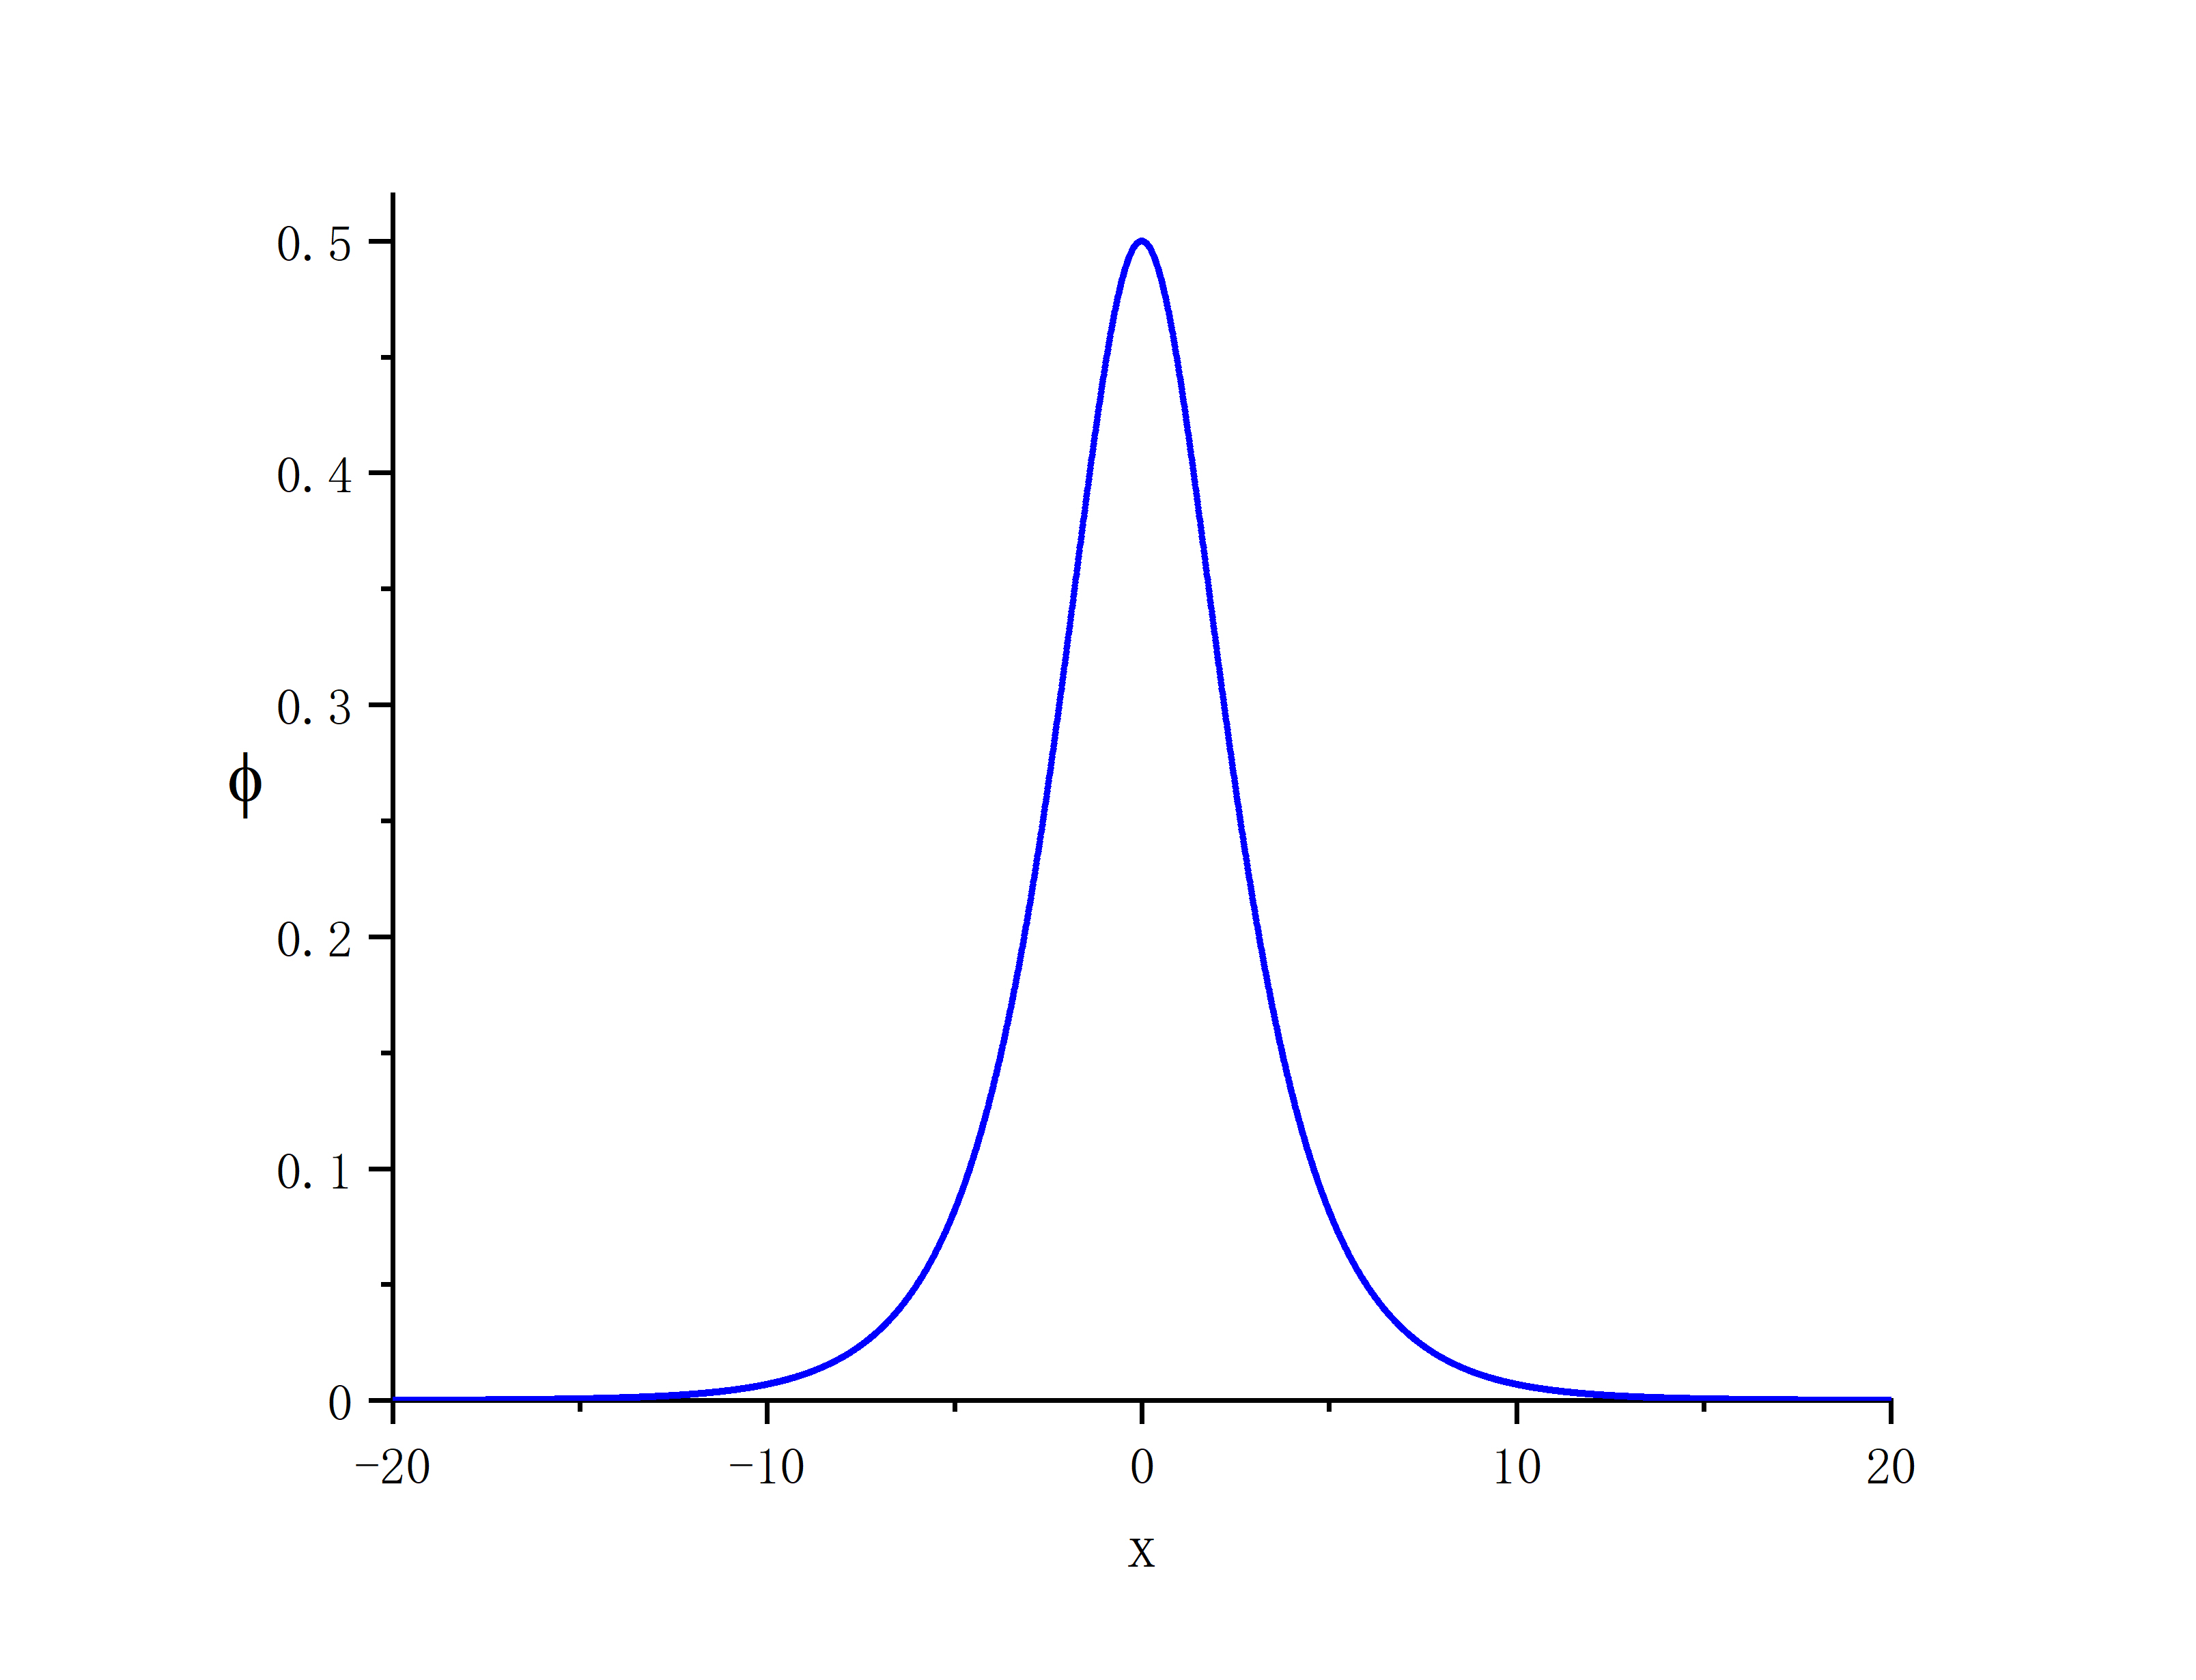
\includegraphics[width=0.8\textwidth]{q3图.jpg}
        \caption{q3图}\label{fig:q3图}
    \end{figure}

    基态本征值$\epsilon=-1.2496\times10^{-1}$.

    总能量无量纲化后变为:(为简便起见,本问解答均省略标度变换后的上标$\tilde X$)

    \begin{align*}
      E=\left\langle \varPsi |H|\varPsi \right\rangle
      &=\int_{-\infty}^\infty(-\frac{n}{2}\phi^*\phi''-\frac{n(n-1)}{2}g|\phi|^4)dx\\
      &=-\frac{n}{2}g^2(n-1)^2\int_{-\infty}^\infty(\tilde{\phi}\tilde{\phi}''+\tilde{\phi}^4)d\tilde{x}
    \end{align*}

    上式积分可用矩形法求出,即

    \[\int_{-\infty}^\infty(\tilde{\phi}\tilde{\phi}''+\tilde{\phi}^4)d\tilde{x}=\sum_{i=1}^n(\tilde{\phi}(\tilde{x}_i)\frac{\tilde{\phi}(\tilde{x}_{i+1})+\tilde{\phi}(\tilde{x}_{i-1})-2\tilde{\phi}(\tilde{x}_i)}{h^2}+\tilde{\phi}(\tilde{x}_i)^4)h\]

    运行结果已由"../data/q3/q3.txt"给出,为$8.33334\times10^{-2}$

    于是总能量为
    \[E=-0.0416667\times g^2n(n-1)^2\]

    \section{第四问解答与结果展示}

    进而离散化后的问题是

    \begin{align*}
      &\begin{pmatrix}
        D_1&-1&0&\cdots&0&0\\
        -1& D_2&-1&\cdots&0&0\\
        0&-1&D_3&\cdots&0&0\\
        \vdots&\vdots&\vdots&\ddots&\vdots&\vdots\\
        0&0&0&\cdots& D_{N-1}&-1\\
        0&0&0&\cdots&-1&D_N
      \end{pmatrix}
      \begin{pmatrix}
        x_1\\
        x_2\\
        x_3\\
        \vdots\\
        x_{N-1}\\
        x_N
      \end{pmatrix}=
      2\epsilon_ih^2
      \begin{pmatrix}
        x_1\\
        x_2\\
        x_3\\
        \vdots\\
        x_{N-1}\\
        x_N
      \end{pmatrix}\\
      &D_k=2+x_k^2h^2-2g(n-1)|\phi_{i-1}(x_k)|^2h^2,k=1,2,3,...,N
    \end{align*}

    这里g(n-1)其实是当作可变参数出现的,我们在程序中用G来表示,为简便起见,无特别说明,下文中G均表示g(n-1)。

    这里同样会遇到基态能量是负值的情况,经验性的,我们取位移p为1-2倍的G。

    计算G=0,1,4,9,16的程序见"../code/q4_calVector.c",结果见"../data/q4/q4_G=X.txt"(X=0,1,4,9,16)。

    可以得到波函数图如下

    \begin{figure}[H]
      \centering
      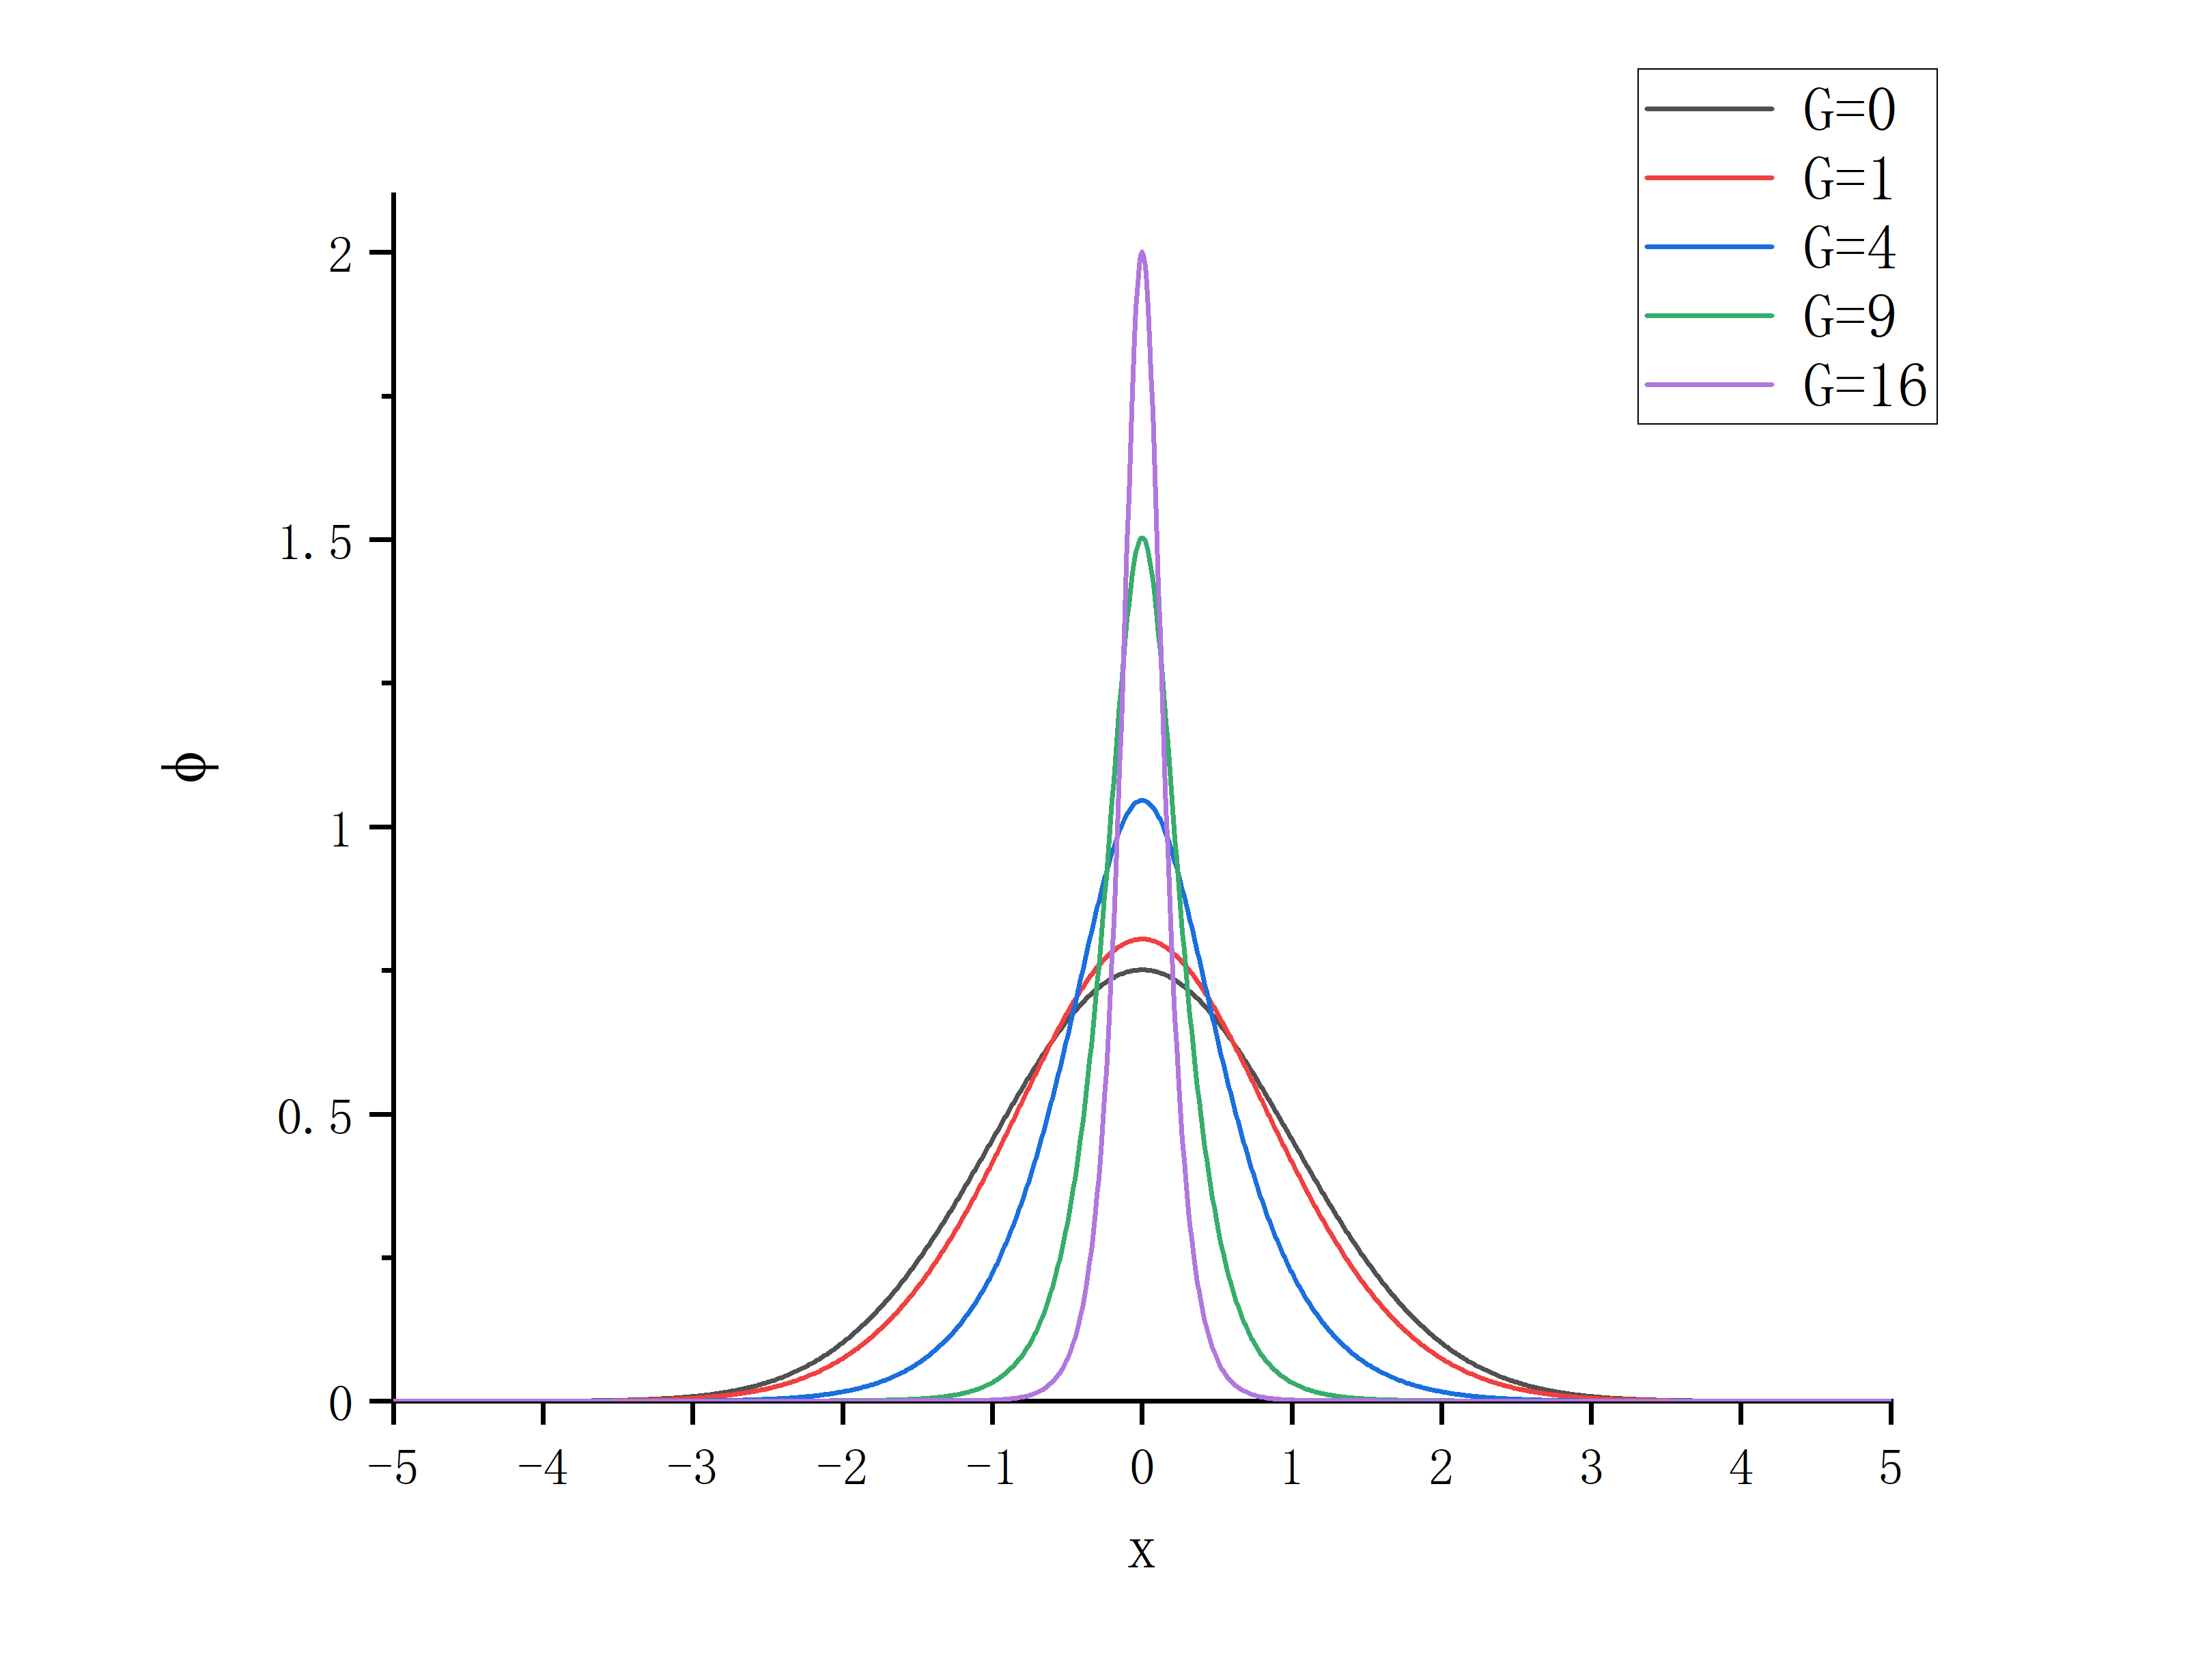
\includegraphics[width=0.8\textwidth]{q4波函数随G变化示意图.jpg}
      \caption{q4波函数随G变化示意图}\label{fig:q4波函数随G变化示意图}
    \end{figure}

    计算本征值的程序见"../code/q4_calValue.c",结果见"../data/q4/q4_values.txt".

    得到本征值随G变化如下
    \begin{figure}[H]
      \centering
      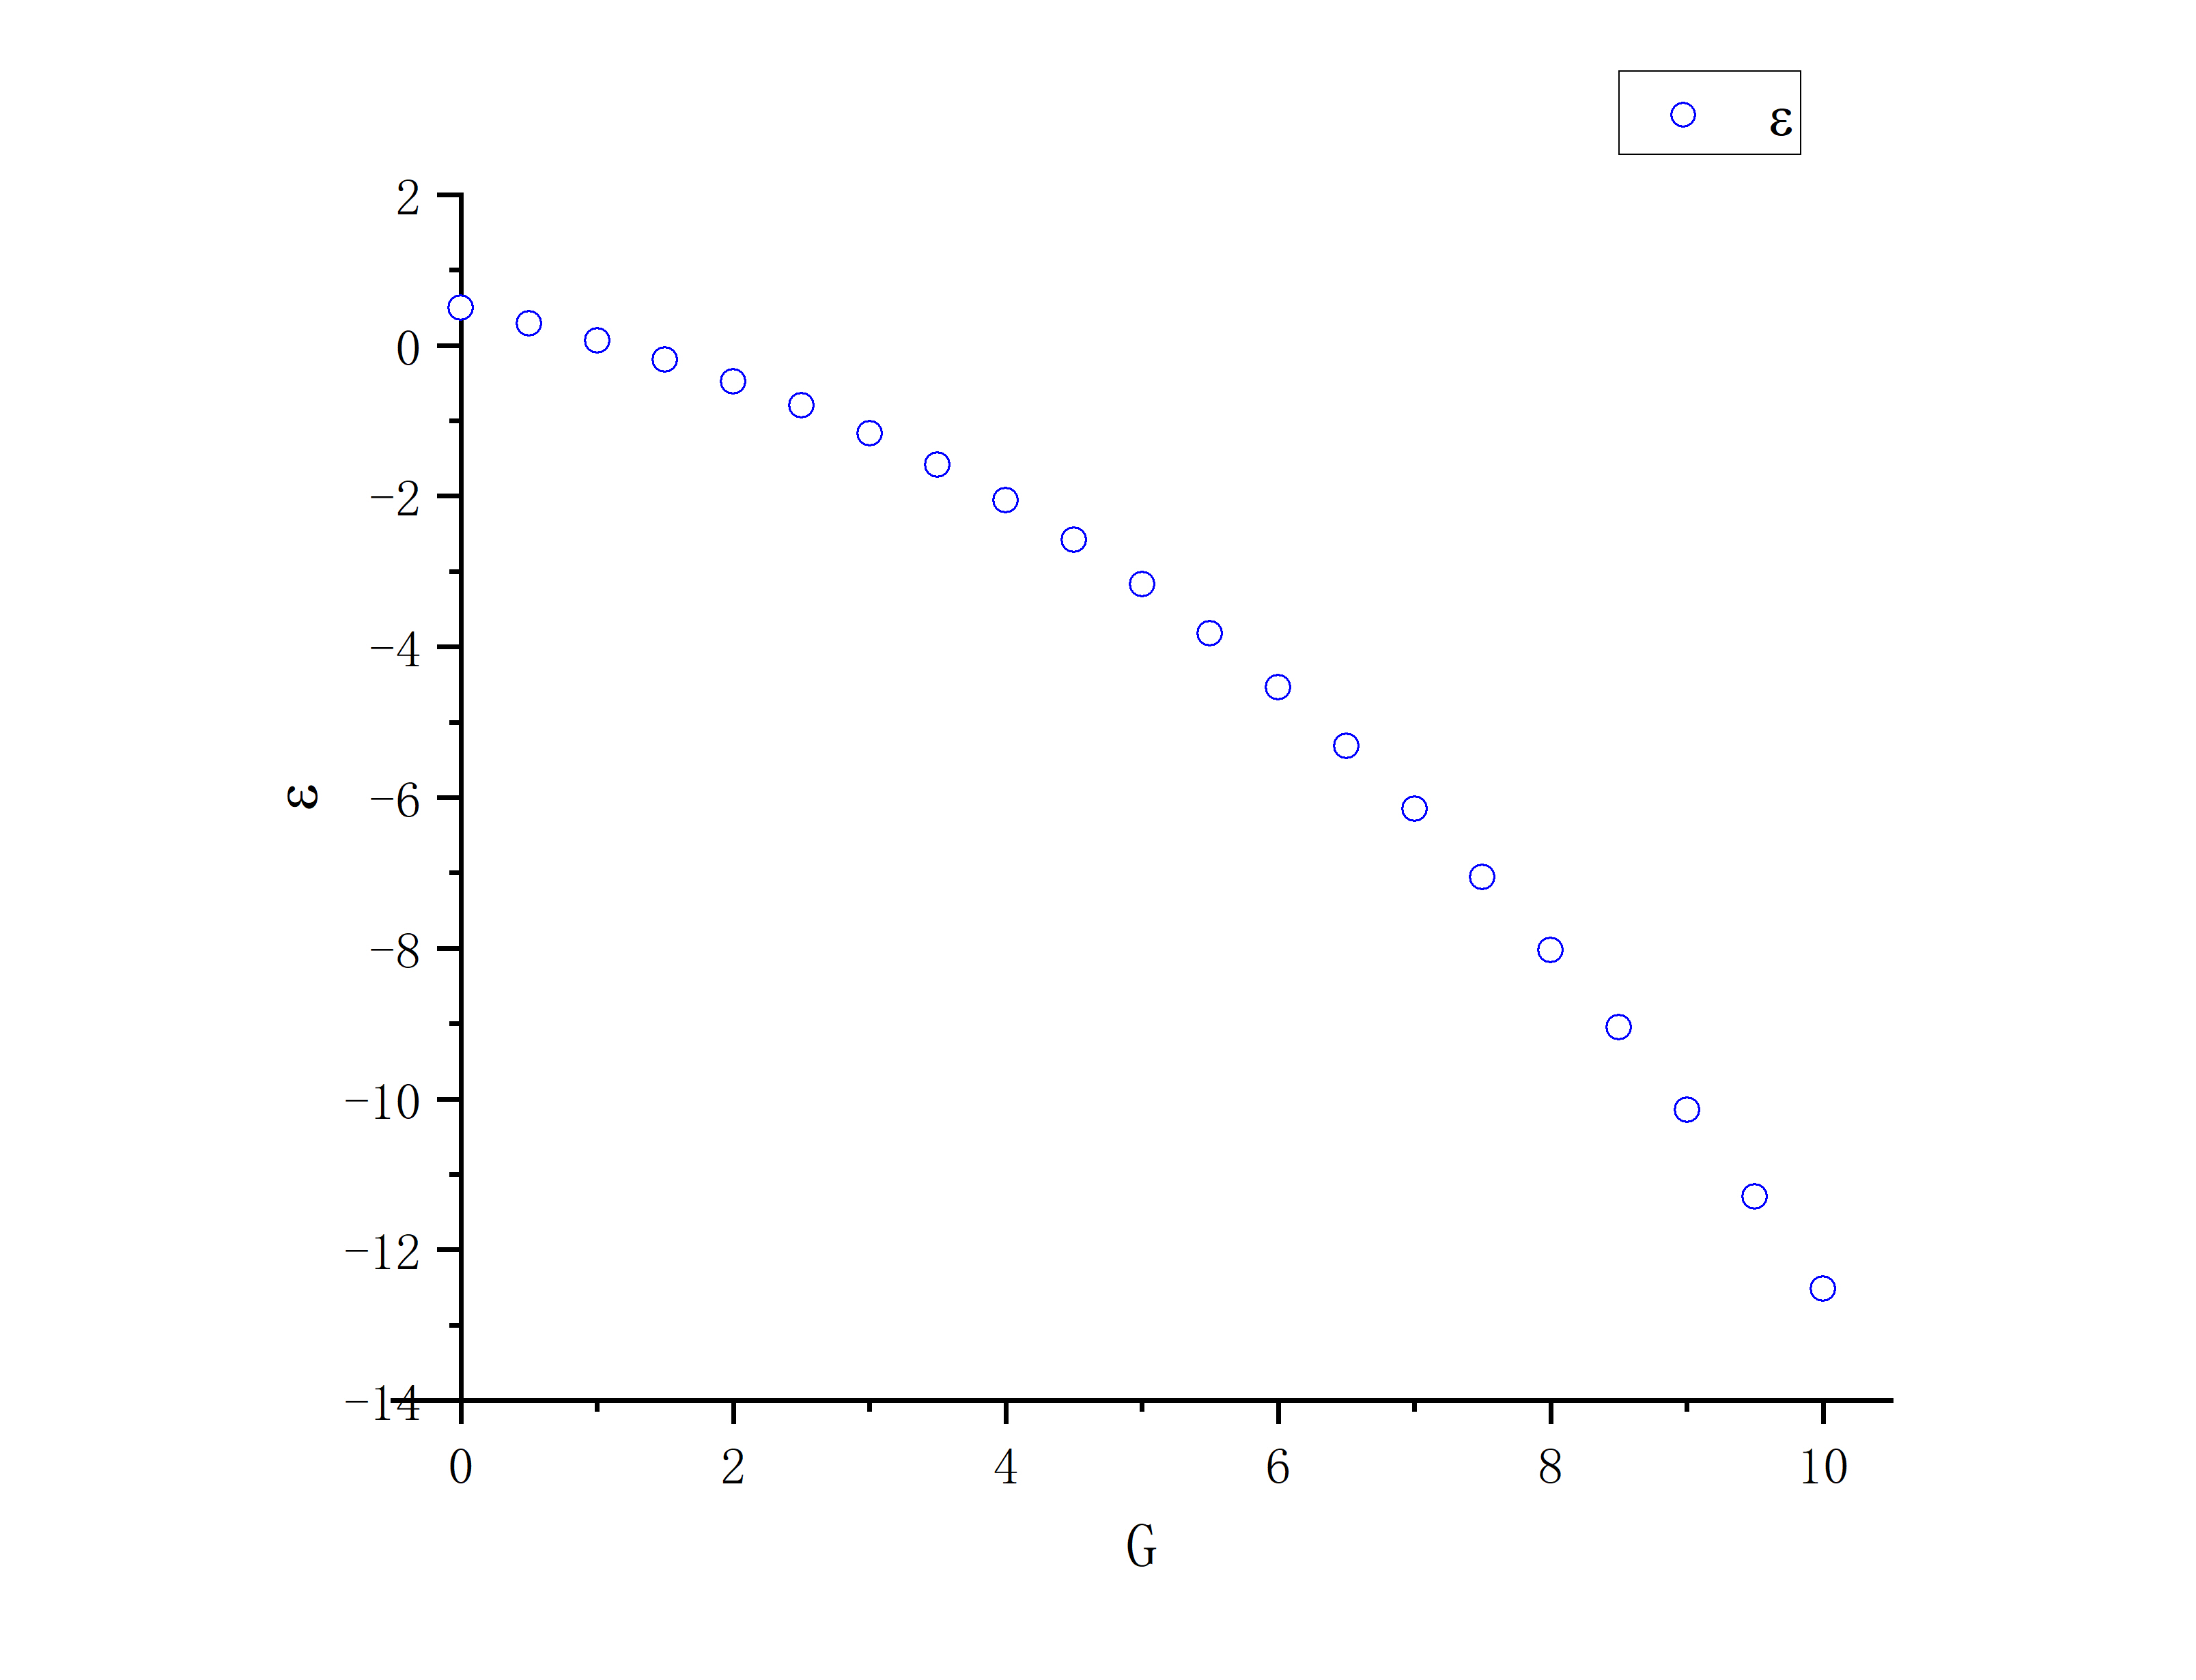
\includegraphics[width=0.8\textwidth]{q4本征值随G变化关系图.jpg}
      \caption{q4本征值随G变化关系图}\label{fig:q4本征值随G变化关系图}
    \end{figure}

    下面说明当G很大时,波函数和本征值结果都趋向q3得到的结果。

    q3,q4相差一个标度变换,因此需要将二者标度统一,下面将q4标度向q3统一。

    已知

    \[\phi(x)\xrightarrow[\text{纵坐标不变,横坐标*G}]{\tilde{x}=Gx}f(\tilde x)\xrightarrow[\text{横坐标不变,纵坐标}/\sqrt{G}]{\tilde{\phi}=f/\sqrt{G}}=\tilde \phi(\tilde x)\]

    对q4中结果做如上操作,把变换后的波函数同q3中的波函数画在一起,得到:

    \begin{figure}[H]
      \centering
      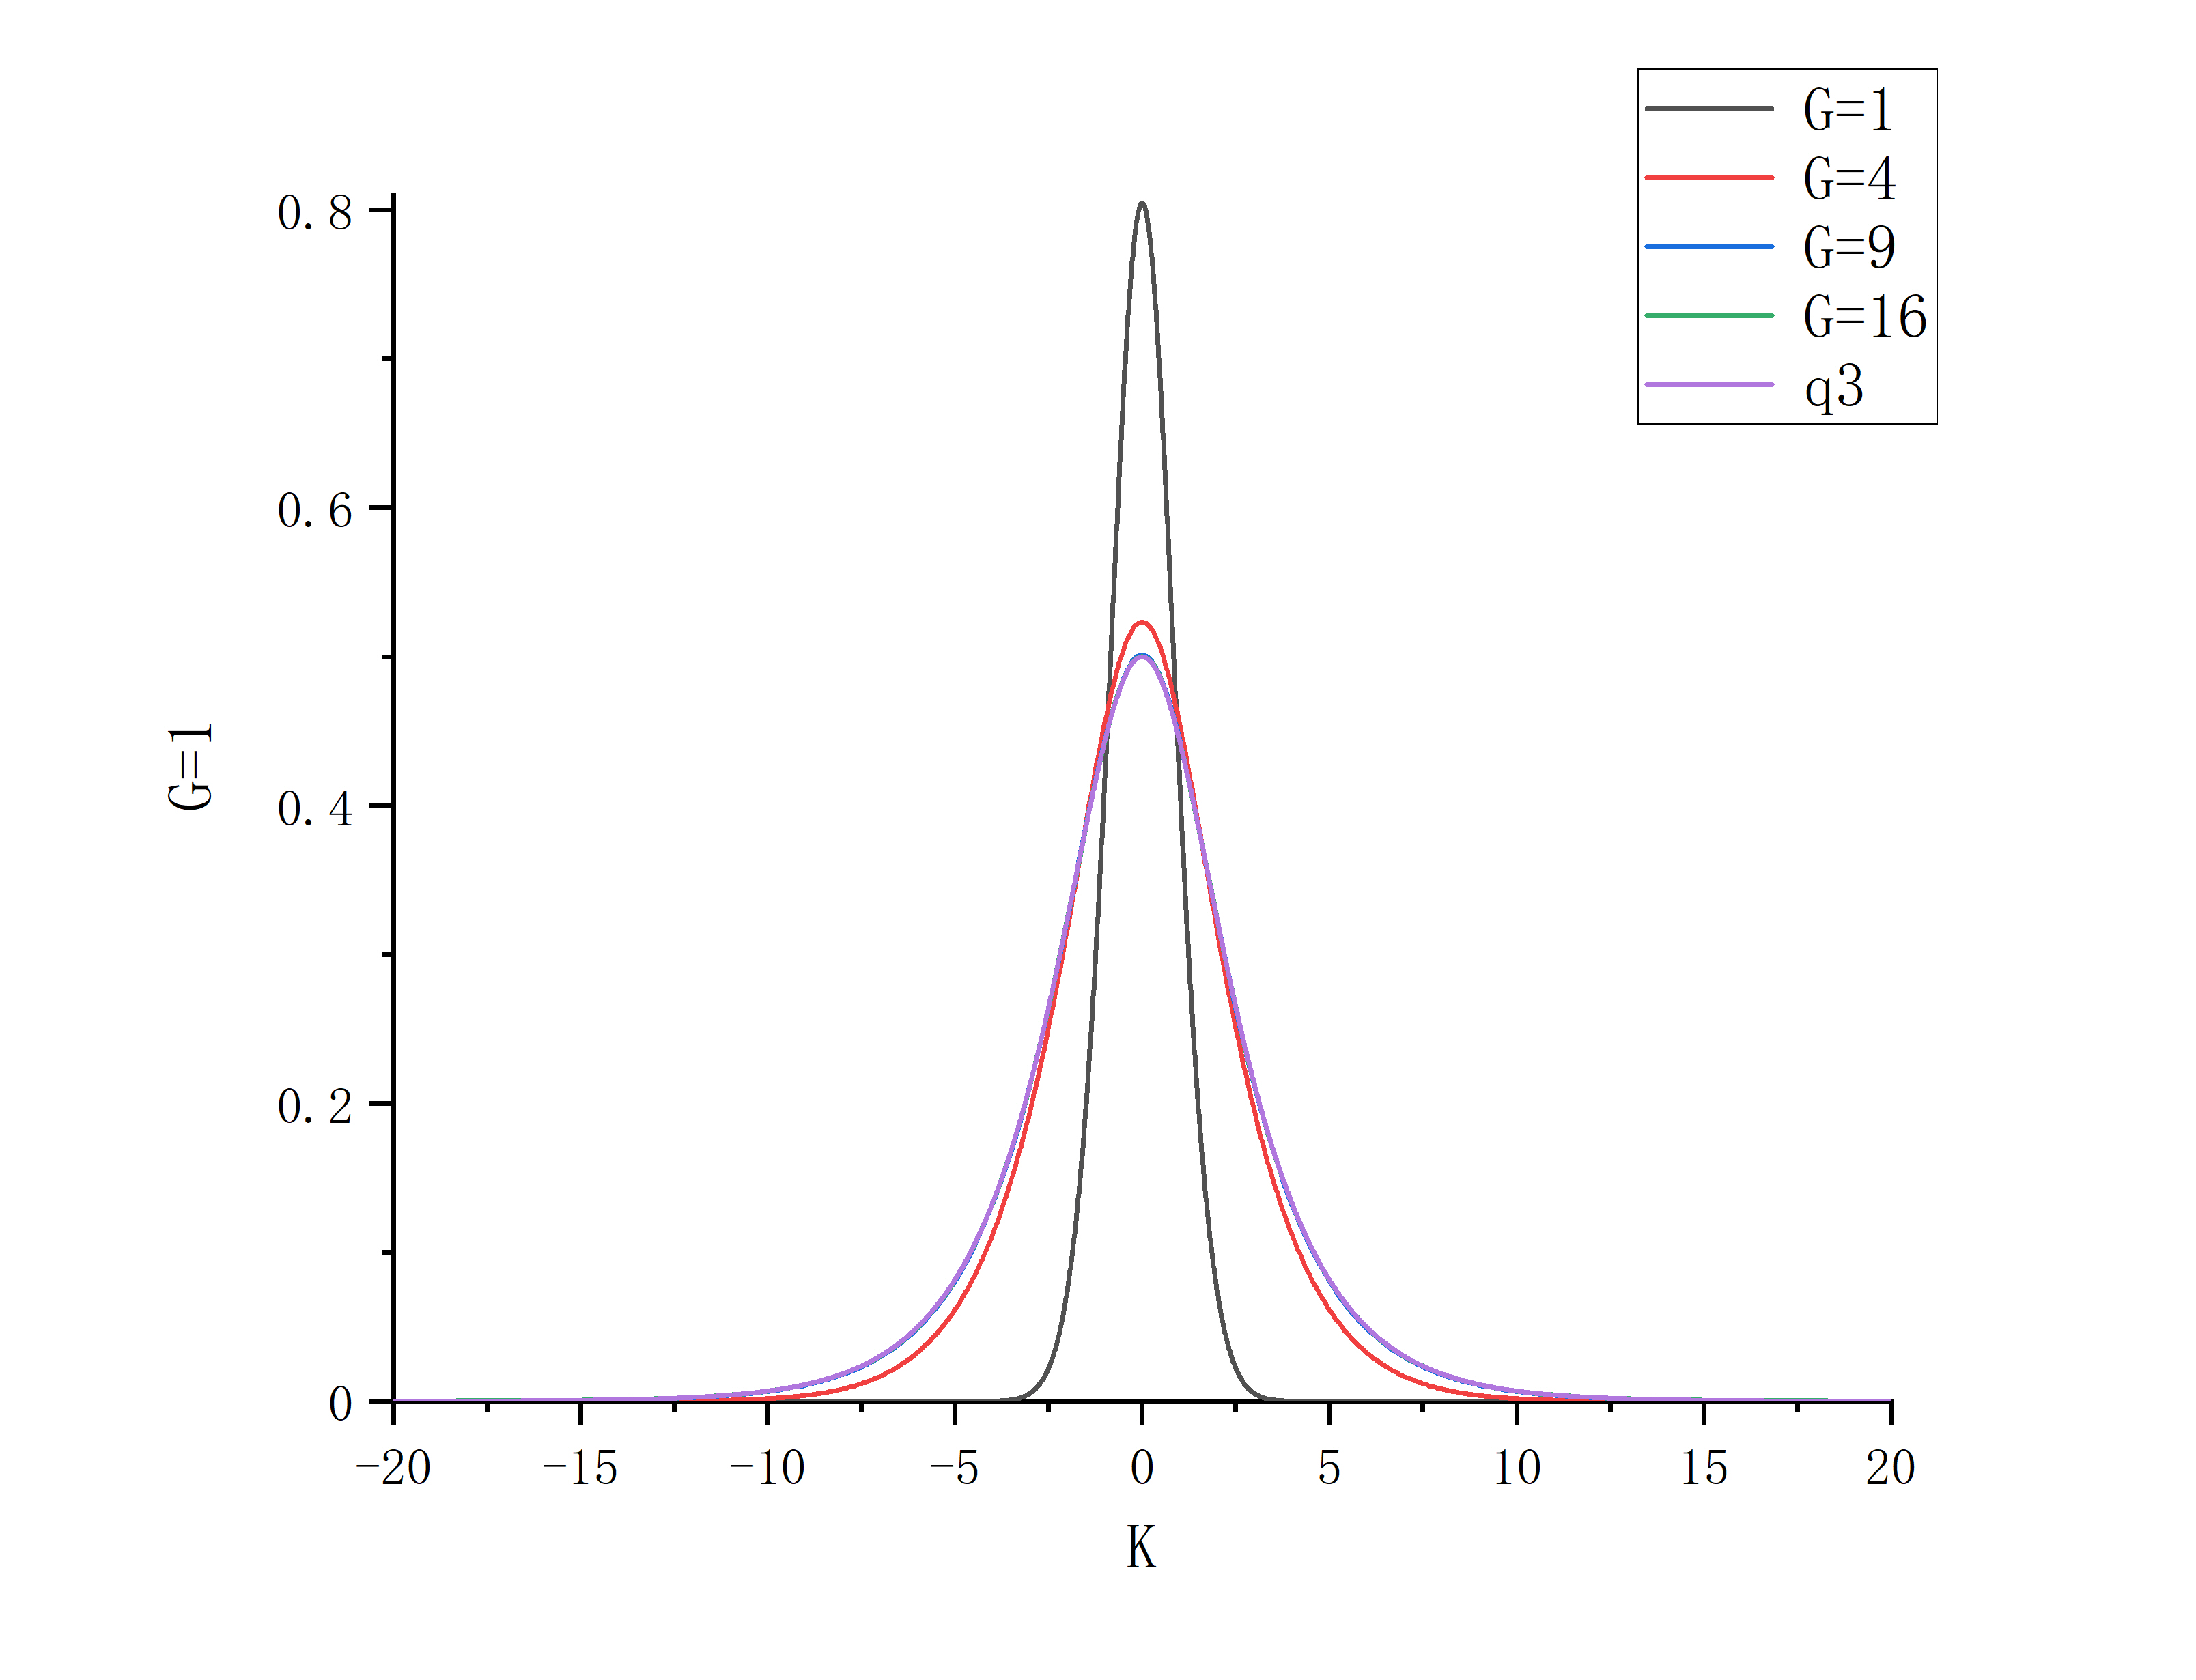
\includegraphics[width=0.8\textwidth]{q4波函数与q3比较.jpg}
      \caption{q4波函数与q3比较}\label{fig:q4波函数与q3比较}
    \end{figure}

    可以看出,G=9和G=16两条线已经完全和q3图重合而看不见了,说明G很大时波函数趋向于q3结果。

    对方程\ref{eq:GPG equation}做标度变换得到

    \begin{equation}\label{eq:标度变换后的GPG eq}
      (-\frac{1}{2}\frac{d^2}{d\tilde x^2}+\frac{1}{2}\frac{\tilde x^2}{G^4}-|\tilde \phi|^2)\tilde \phi=\frac\epsilon {G^2}\tilde \phi
    \end{equation}
     
    于是第三问中的$\tilde\epsilon$与第四问中的$\epsilon$关系为$\tilde\epsilon=\epsilon/G^2$

    于是将q4中的数据按上述方式变换后得到下图(去除了G=0的点)

    \begin{figure}[H]
      \centering
      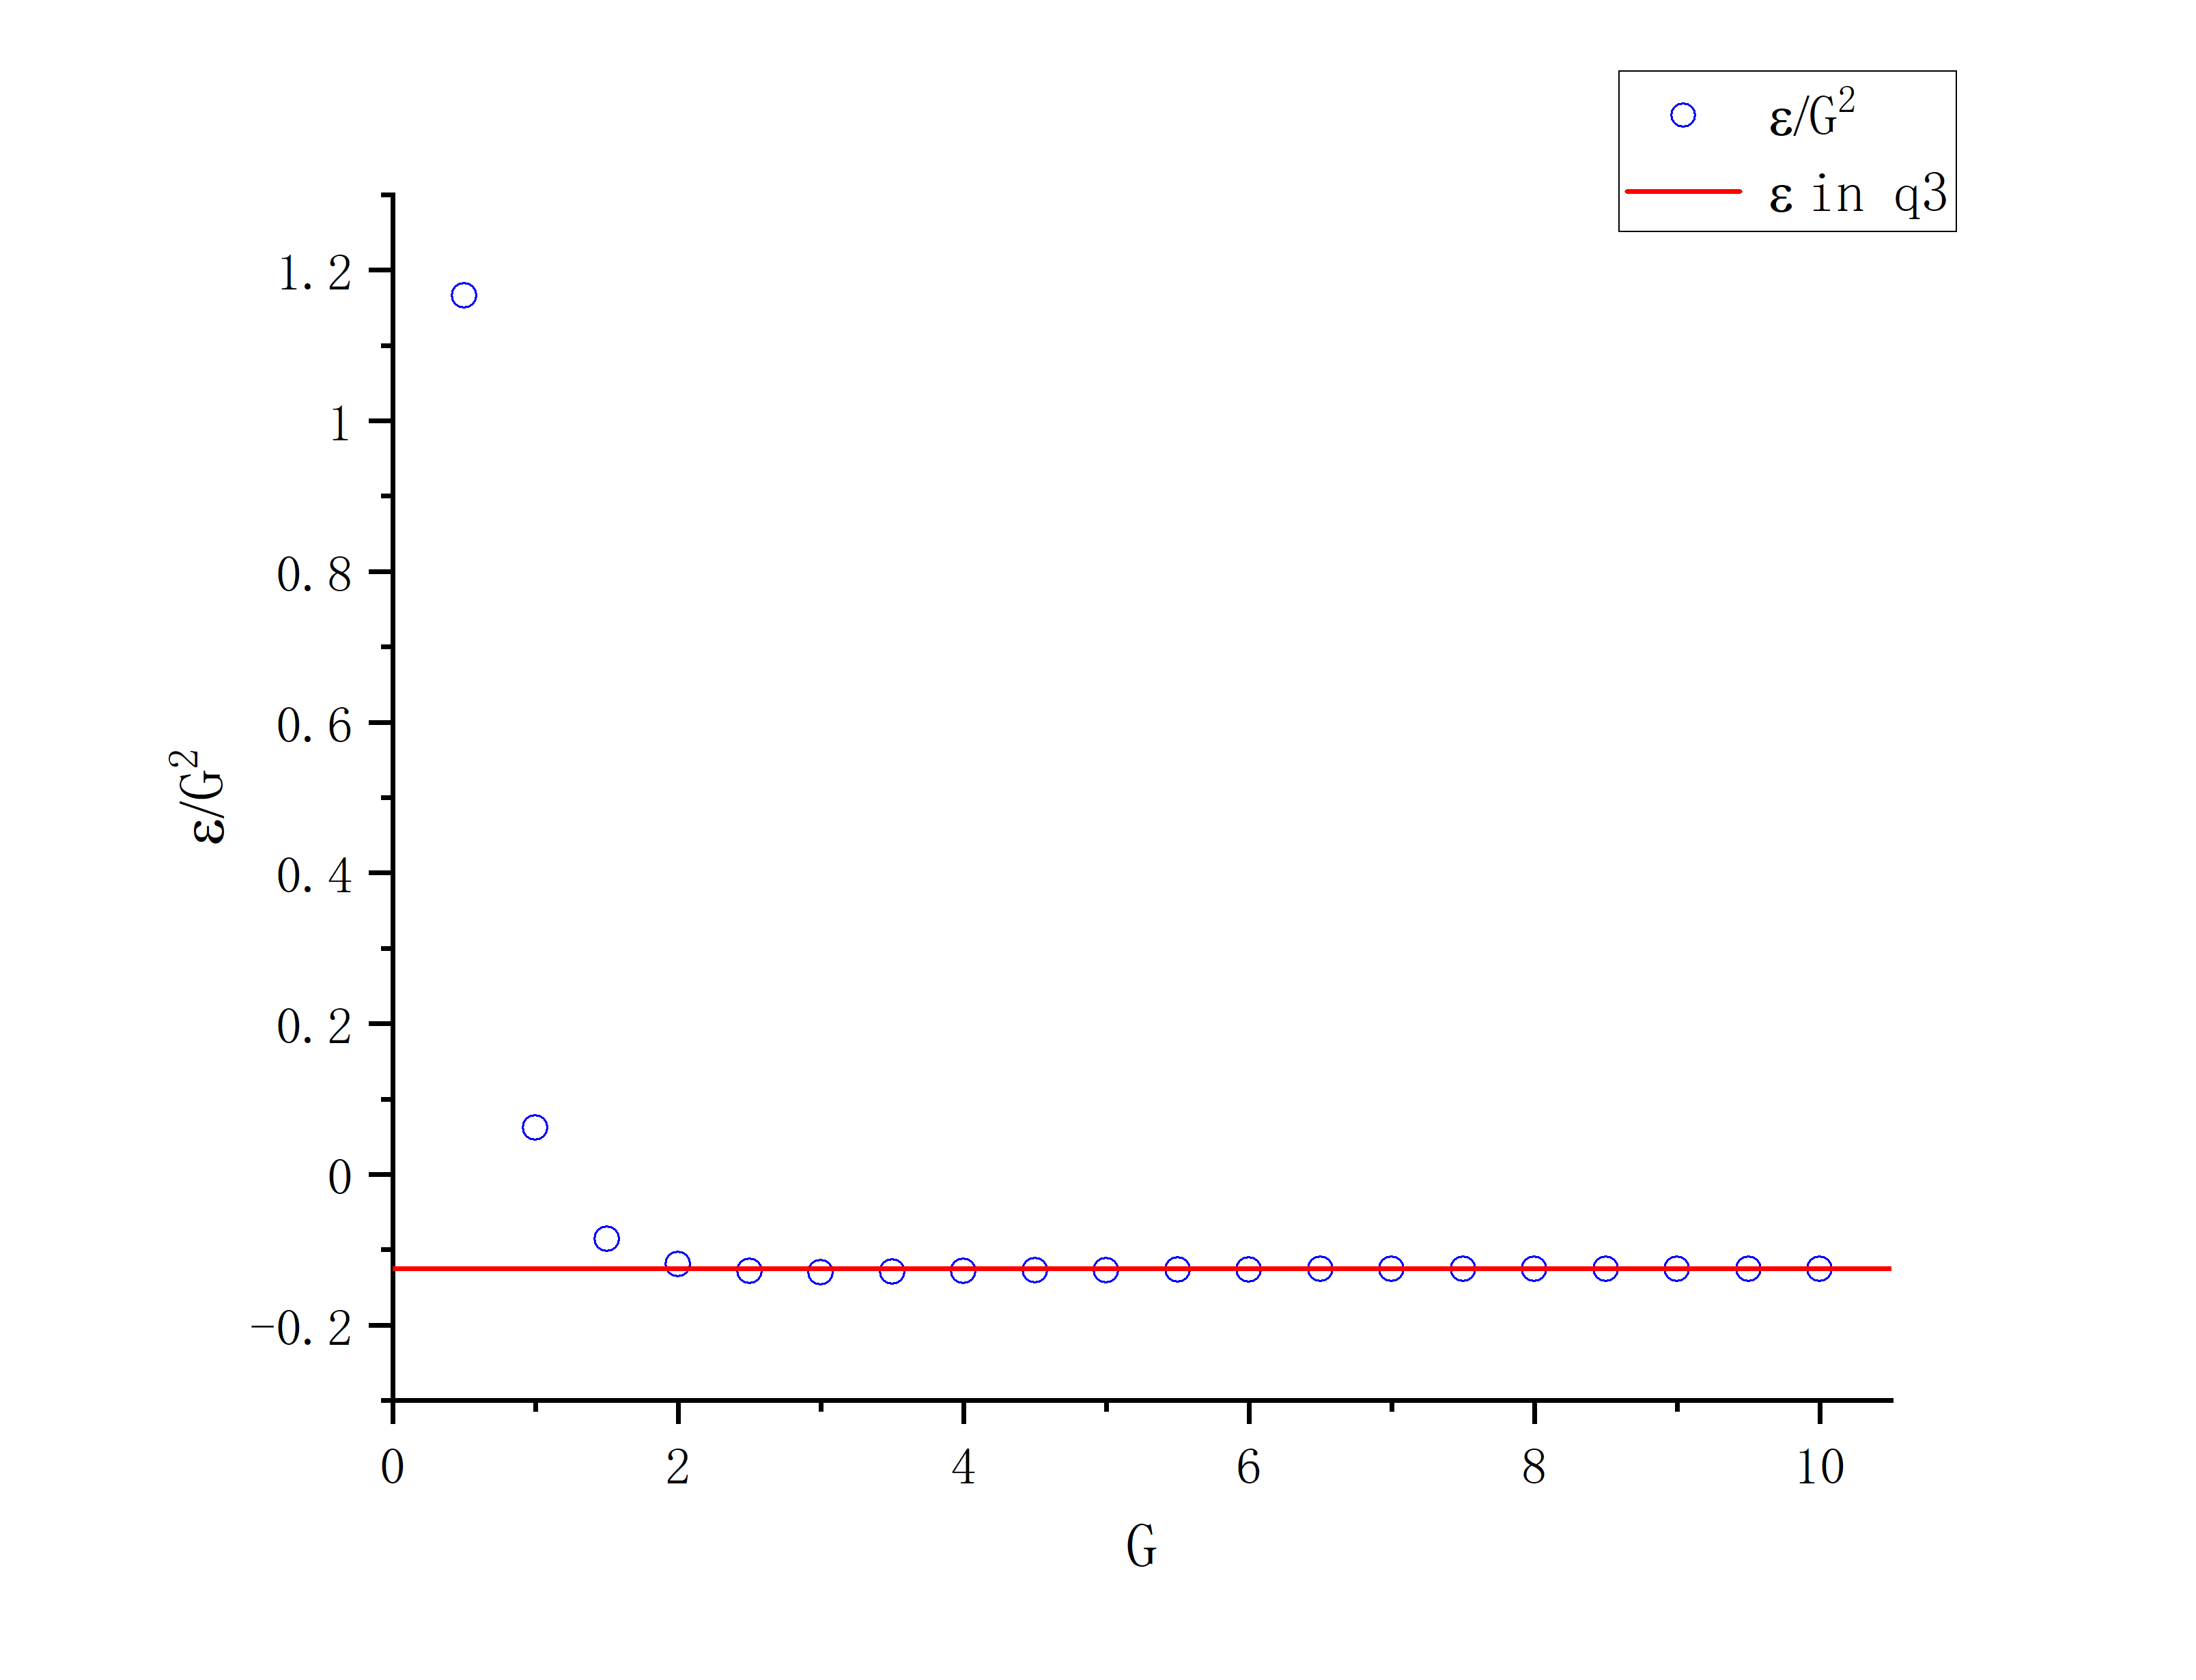
\includegraphics[width=0.8\textwidth]{q4本征值与q3比较.jpg}
      \caption{q4本征值与q3比较}\label{fig:q4本征值与q3比较}
    \end{figure}

    其中红线是第三问中的$\epsilon$值,可以看出,当G增大时,第四问的结果很快地收敛到第三问。

    第四问结果和第三问统一标度后很快地收敛到第三问,这可以从原始方程看出端倪。方程\ref{eq:标度变换后的GPG eq}中G增大后,由于势能项除以了$G^4$,贡献将迅速变小,自然就和第三问中无势能情况一致了。

    \section{第五问解答与结果展示}

    本问与上问类似,只需将G取为负数即可,而且,本问基态能量恒大于0,所以反幂法位移取成0即可。

     计算G=0,-0.5,-1,-1.5,-2的程序见"../code/q5_calVector.c",结果见"../data/q5/q5_G=X.txt"(X=0.,-0.5,-1.0,-1.5,-2.0)。

     得到下图

     \begin{figure}[H]
      \centering
      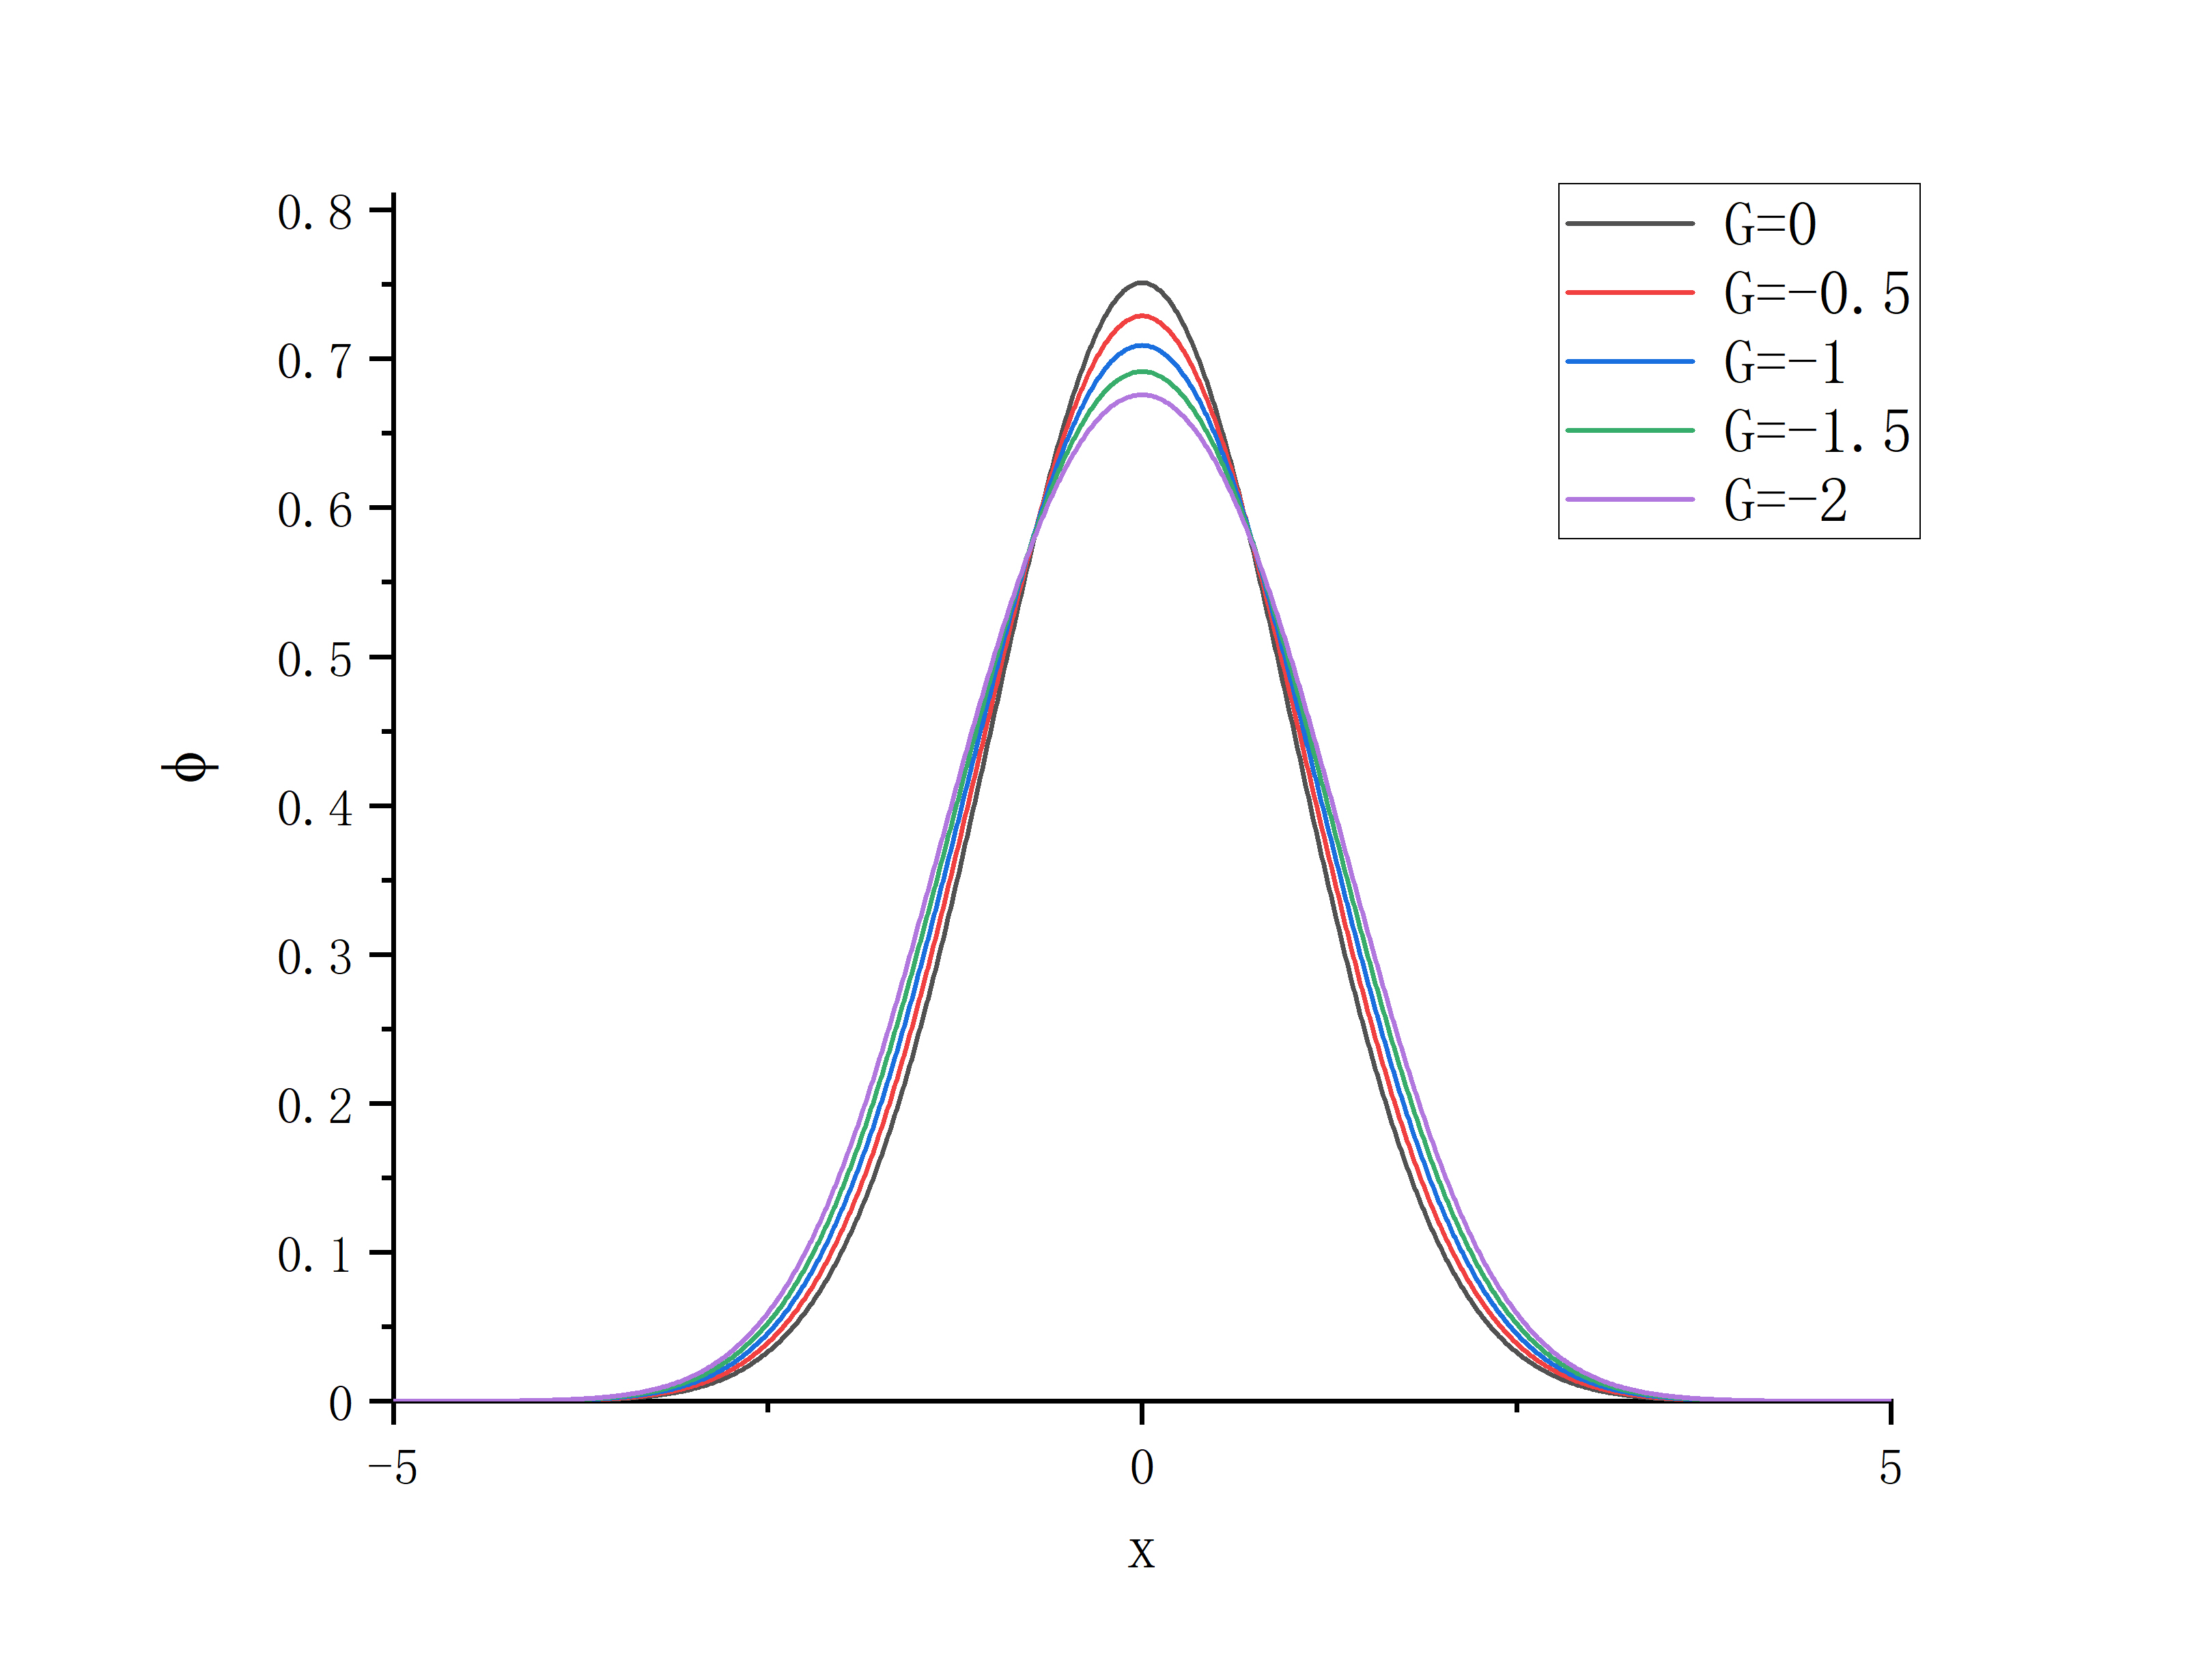
\includegraphics[width=0.8\textwidth]{q5波函数随G变化示意图.jpg}
      \caption{q5波函数随G变化示意图}\label{fig:q5波函数随G变化示意图}
    \end{figure}

     计算本征值的程序见"../code/q4_calValue.c",结果见"../data/q4/q4_values.txt".

     得到下图

     \begin{figure}[H]
      \centering
      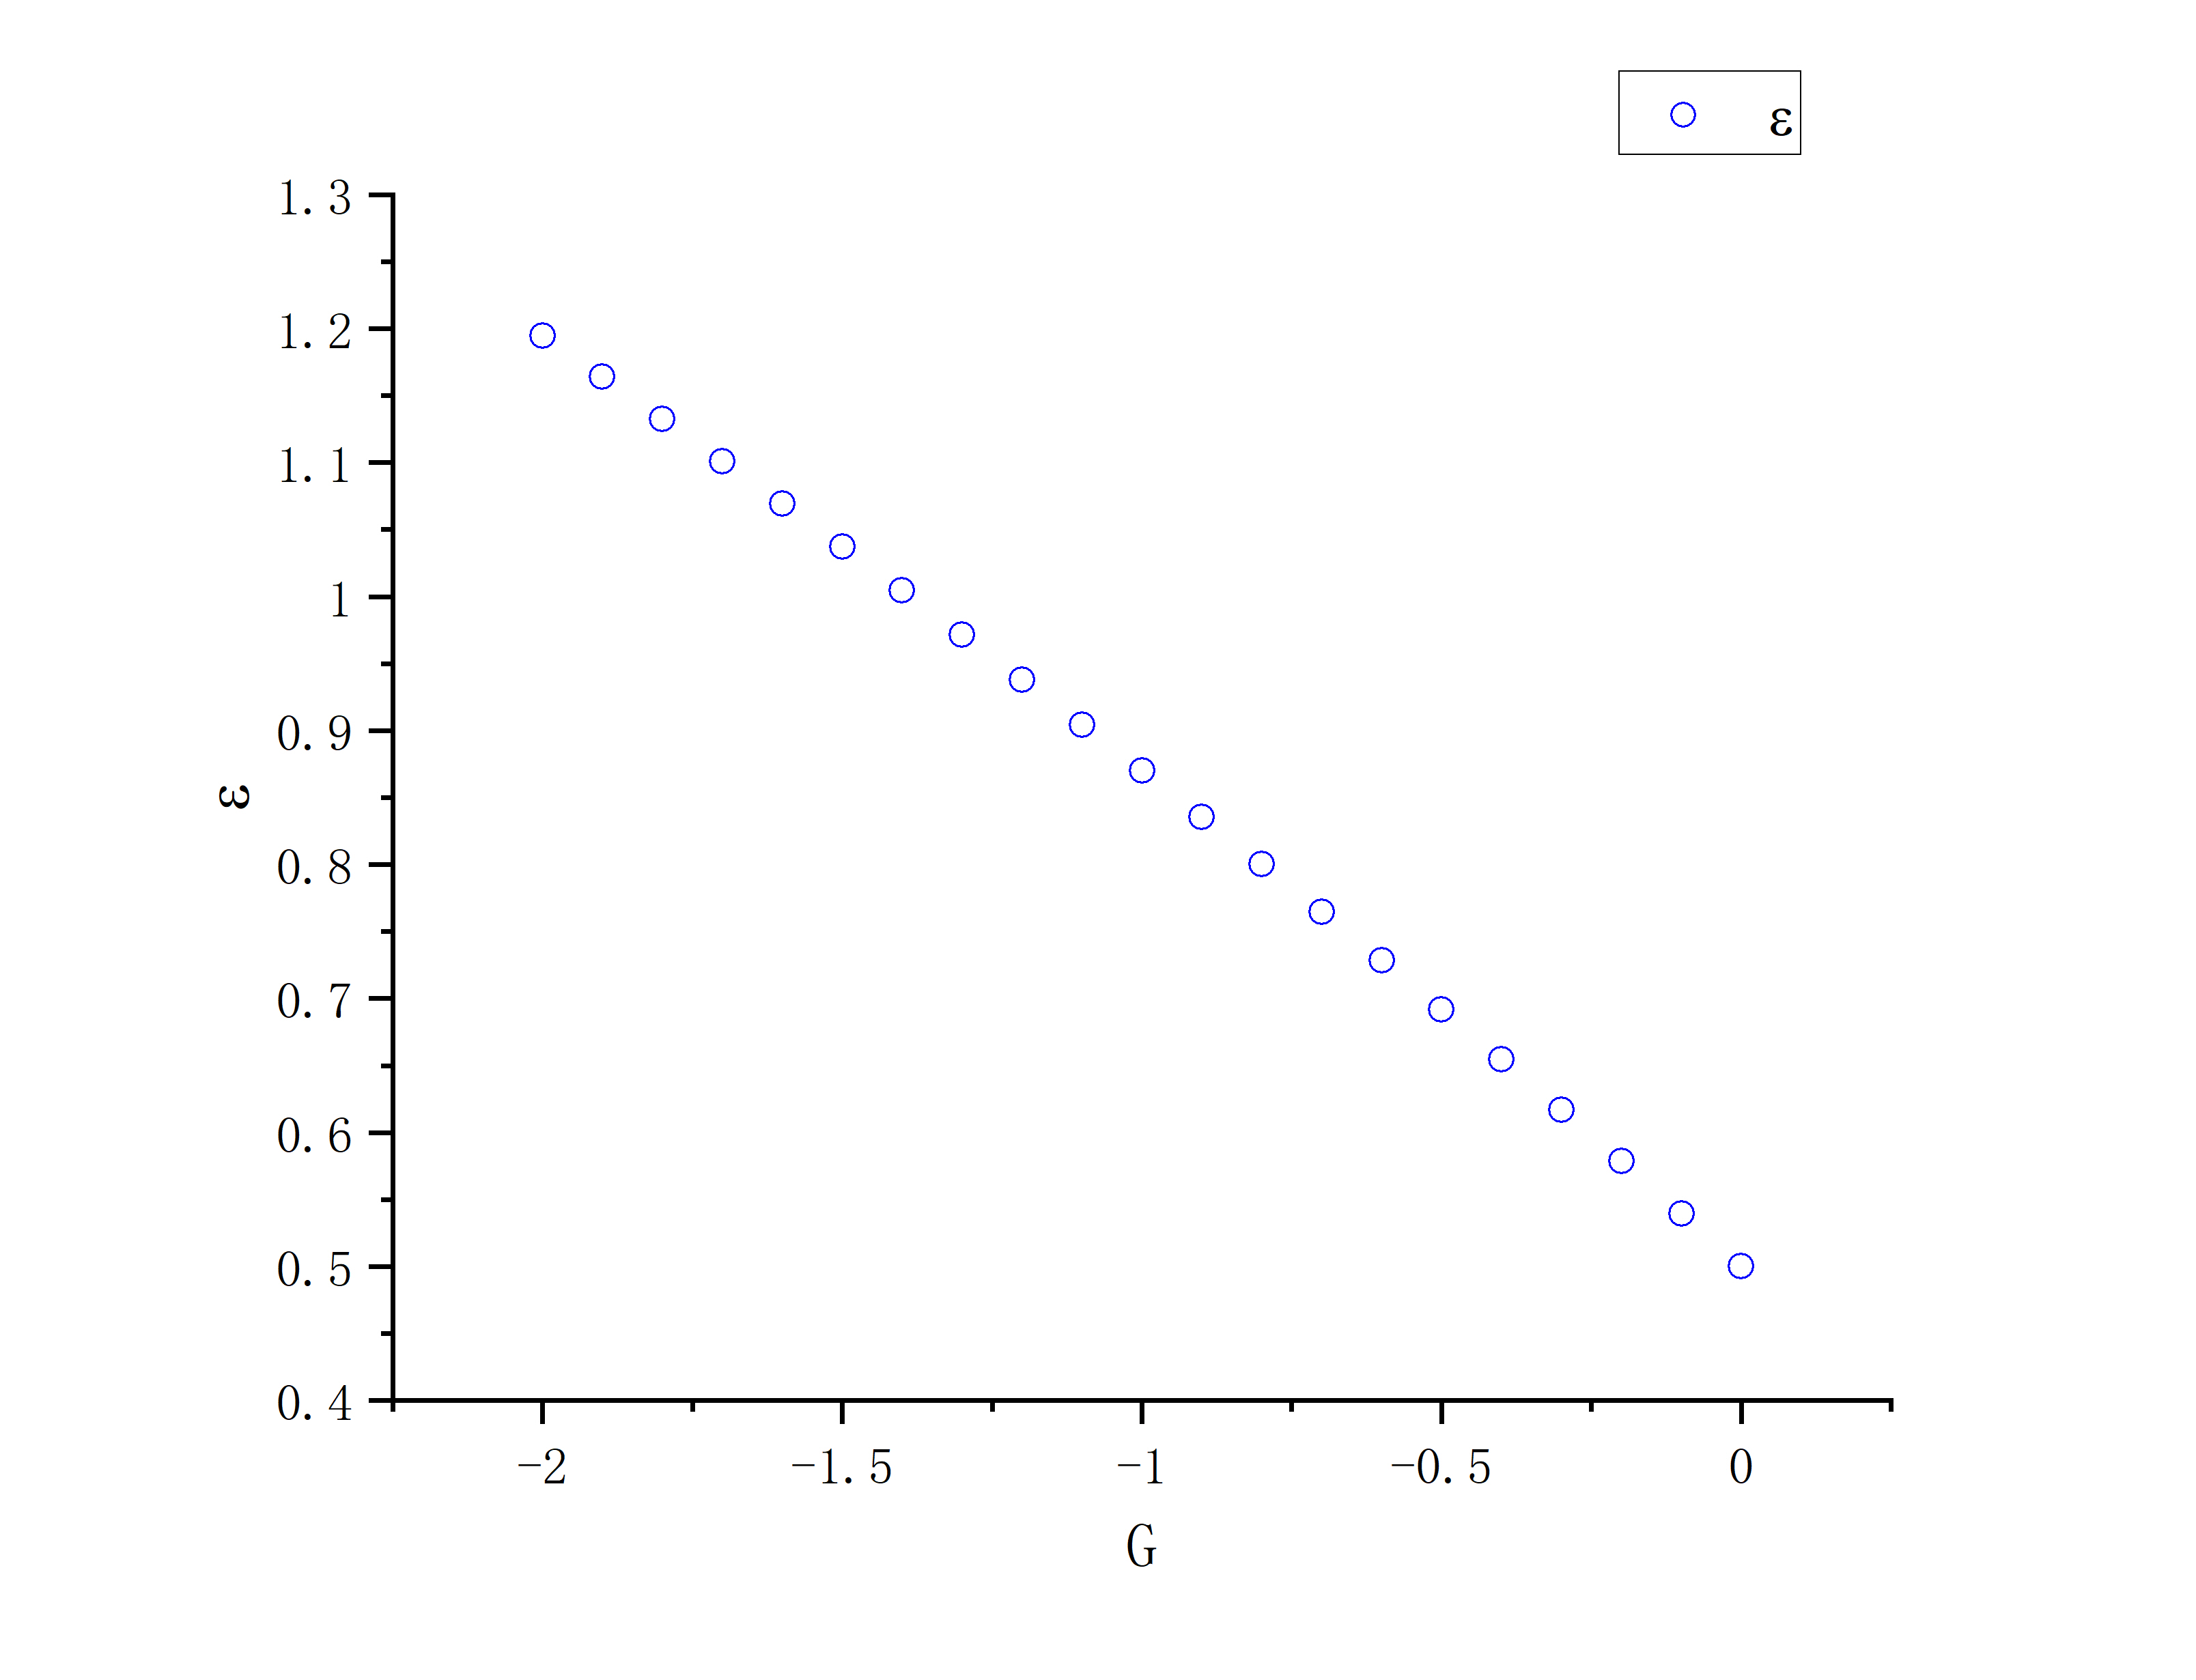
\includegraphics[width=0.8\textwidth]{q5本征值随G变化示意图.jpg}
      \caption{q5本征值随G变化示意图}\label{fig:q5本征值随G变化示意图}
    \end{figure}

    将题目所给的近似解波函数归一化得到波函数近似解为

    \begin{align*}
      \phi(x)=\frac{\sqrt{1-\frac{x^2}{2\epsilon}}}{\sqrt{\frac{4}{3}\sqrt{2\epsilon}}}\eta(\sqrt{2\epsilon}-|x|)
    \end{align*}

    其中$\eta(x)$是阶跃函数。

    将数值得到的$\epsilon$代入可以得到不同G值下近似波函数,和精确求解的波函数画在一起得到下图。

    \begin{figure}[H]
      \centering
      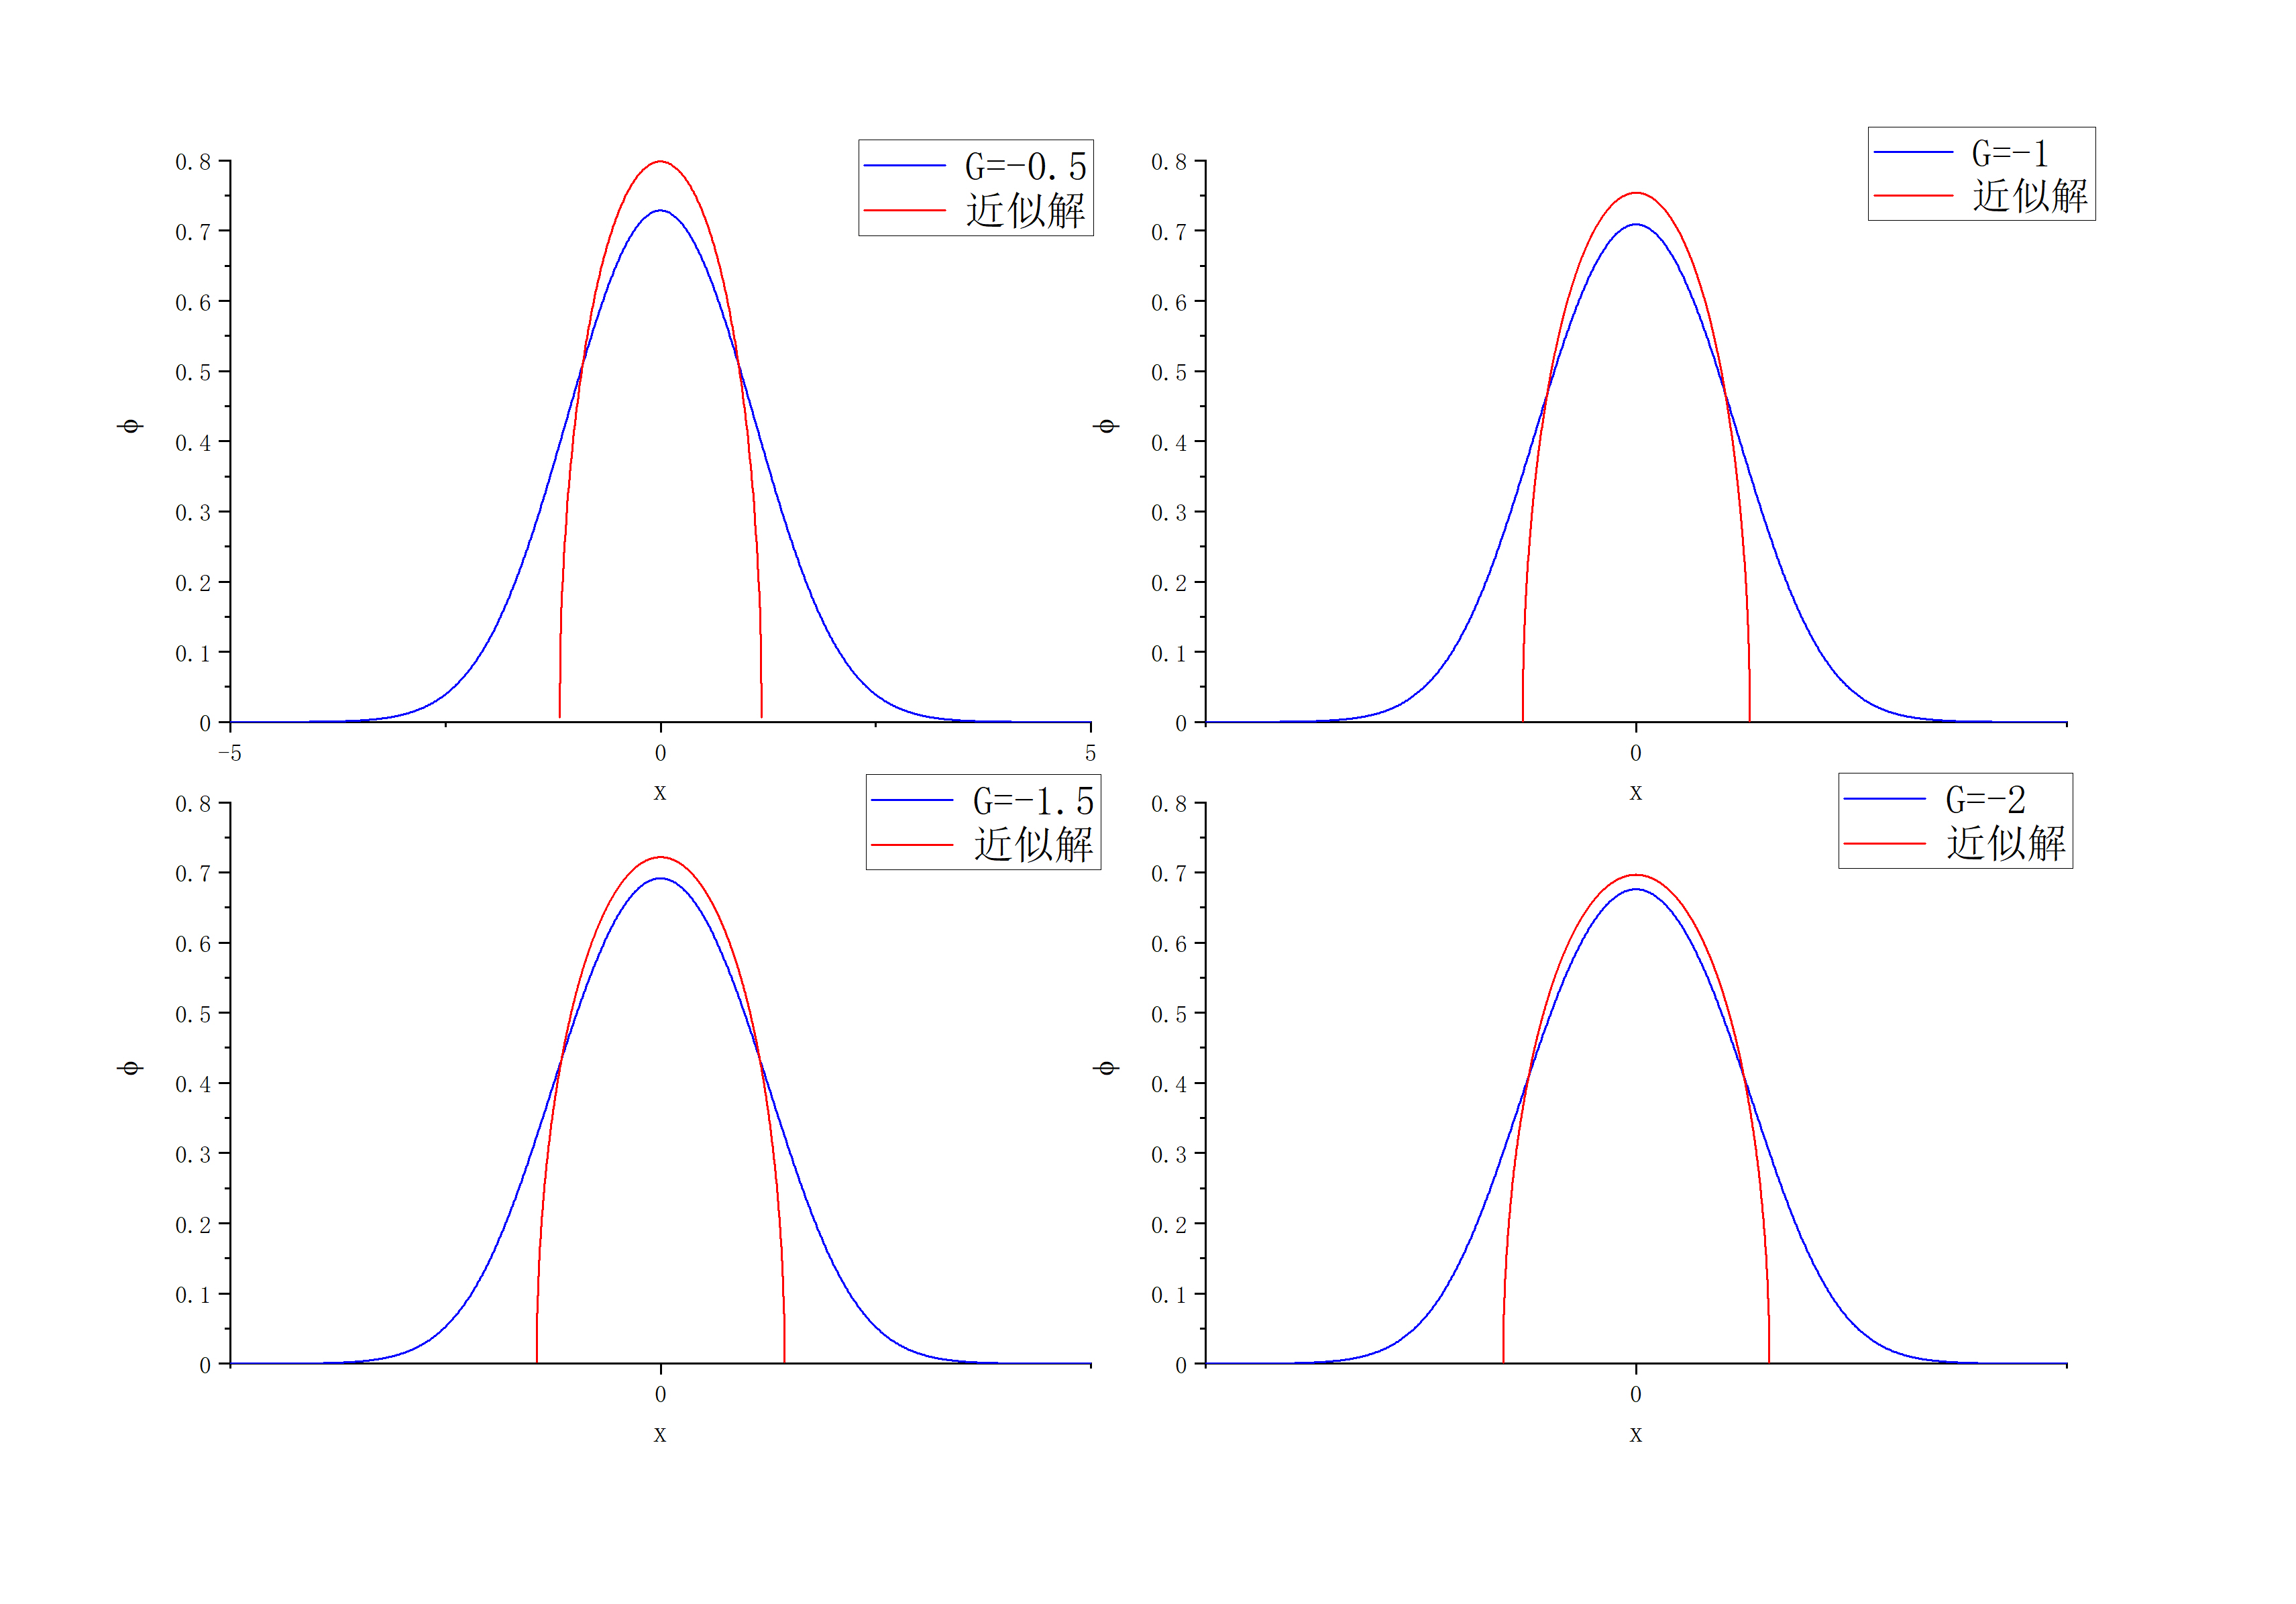
\includegraphics[width=0.8\textwidth]{q5精确解和近似解对比图.jpg}
      \caption{q5精确解和近似解对比图}\label{fig:q5精确解和近似解对比图}
    \end{figure}

    可以看出,当|G|不断增大时,近似解的确在向精确解靠拢,尤其是x=0附近。这说明,在波函数取值最大的地方,近似解和精确解在|G|很大时相近。然而,无论|G|多么大,近似解一定会在某处截断,而精确解会逐渐趋向于0,于是,精确解和近似解在远离原点的位置差异较大。但是我们仍然认为|G|充分大时\textbf{近似解合理},因为在实际计算可观测量平均值时,x=0附近的波函数是积分的主要贡献项,远离原点的部分近似解和精确解的差异给可观测量计算带来的差异很小,由于近似解和精确解在原点附近贴合,那么这个精确解在计算平均值意义上是有意义的、合理的。

    之所以|G|很大时在原点附近舍去动能项可以得到波函数的很好近似,是因为G代表粒子间排斥力的强度,当|G|很大时,在原点附近粒子排斥势很强,能量守恒,于是动能很小,可以舍去。

    \section{思考题}

    需要指出的是,在第五问中当G靠近-2时,波函数和特征值收敛会变得困难,以至于经过足够多迭代次数,相邻两次迭代的特征值相对偏差和波函数的距离会趋向于一个正的常数,而不是0,如下图所示\footnote{图中数据可由"../code/plot_iteration.c"打出,输出文件见"../data/extra/plot_iteration_G=-2.txt"}

    \begin{figure}[H]
      \centering
      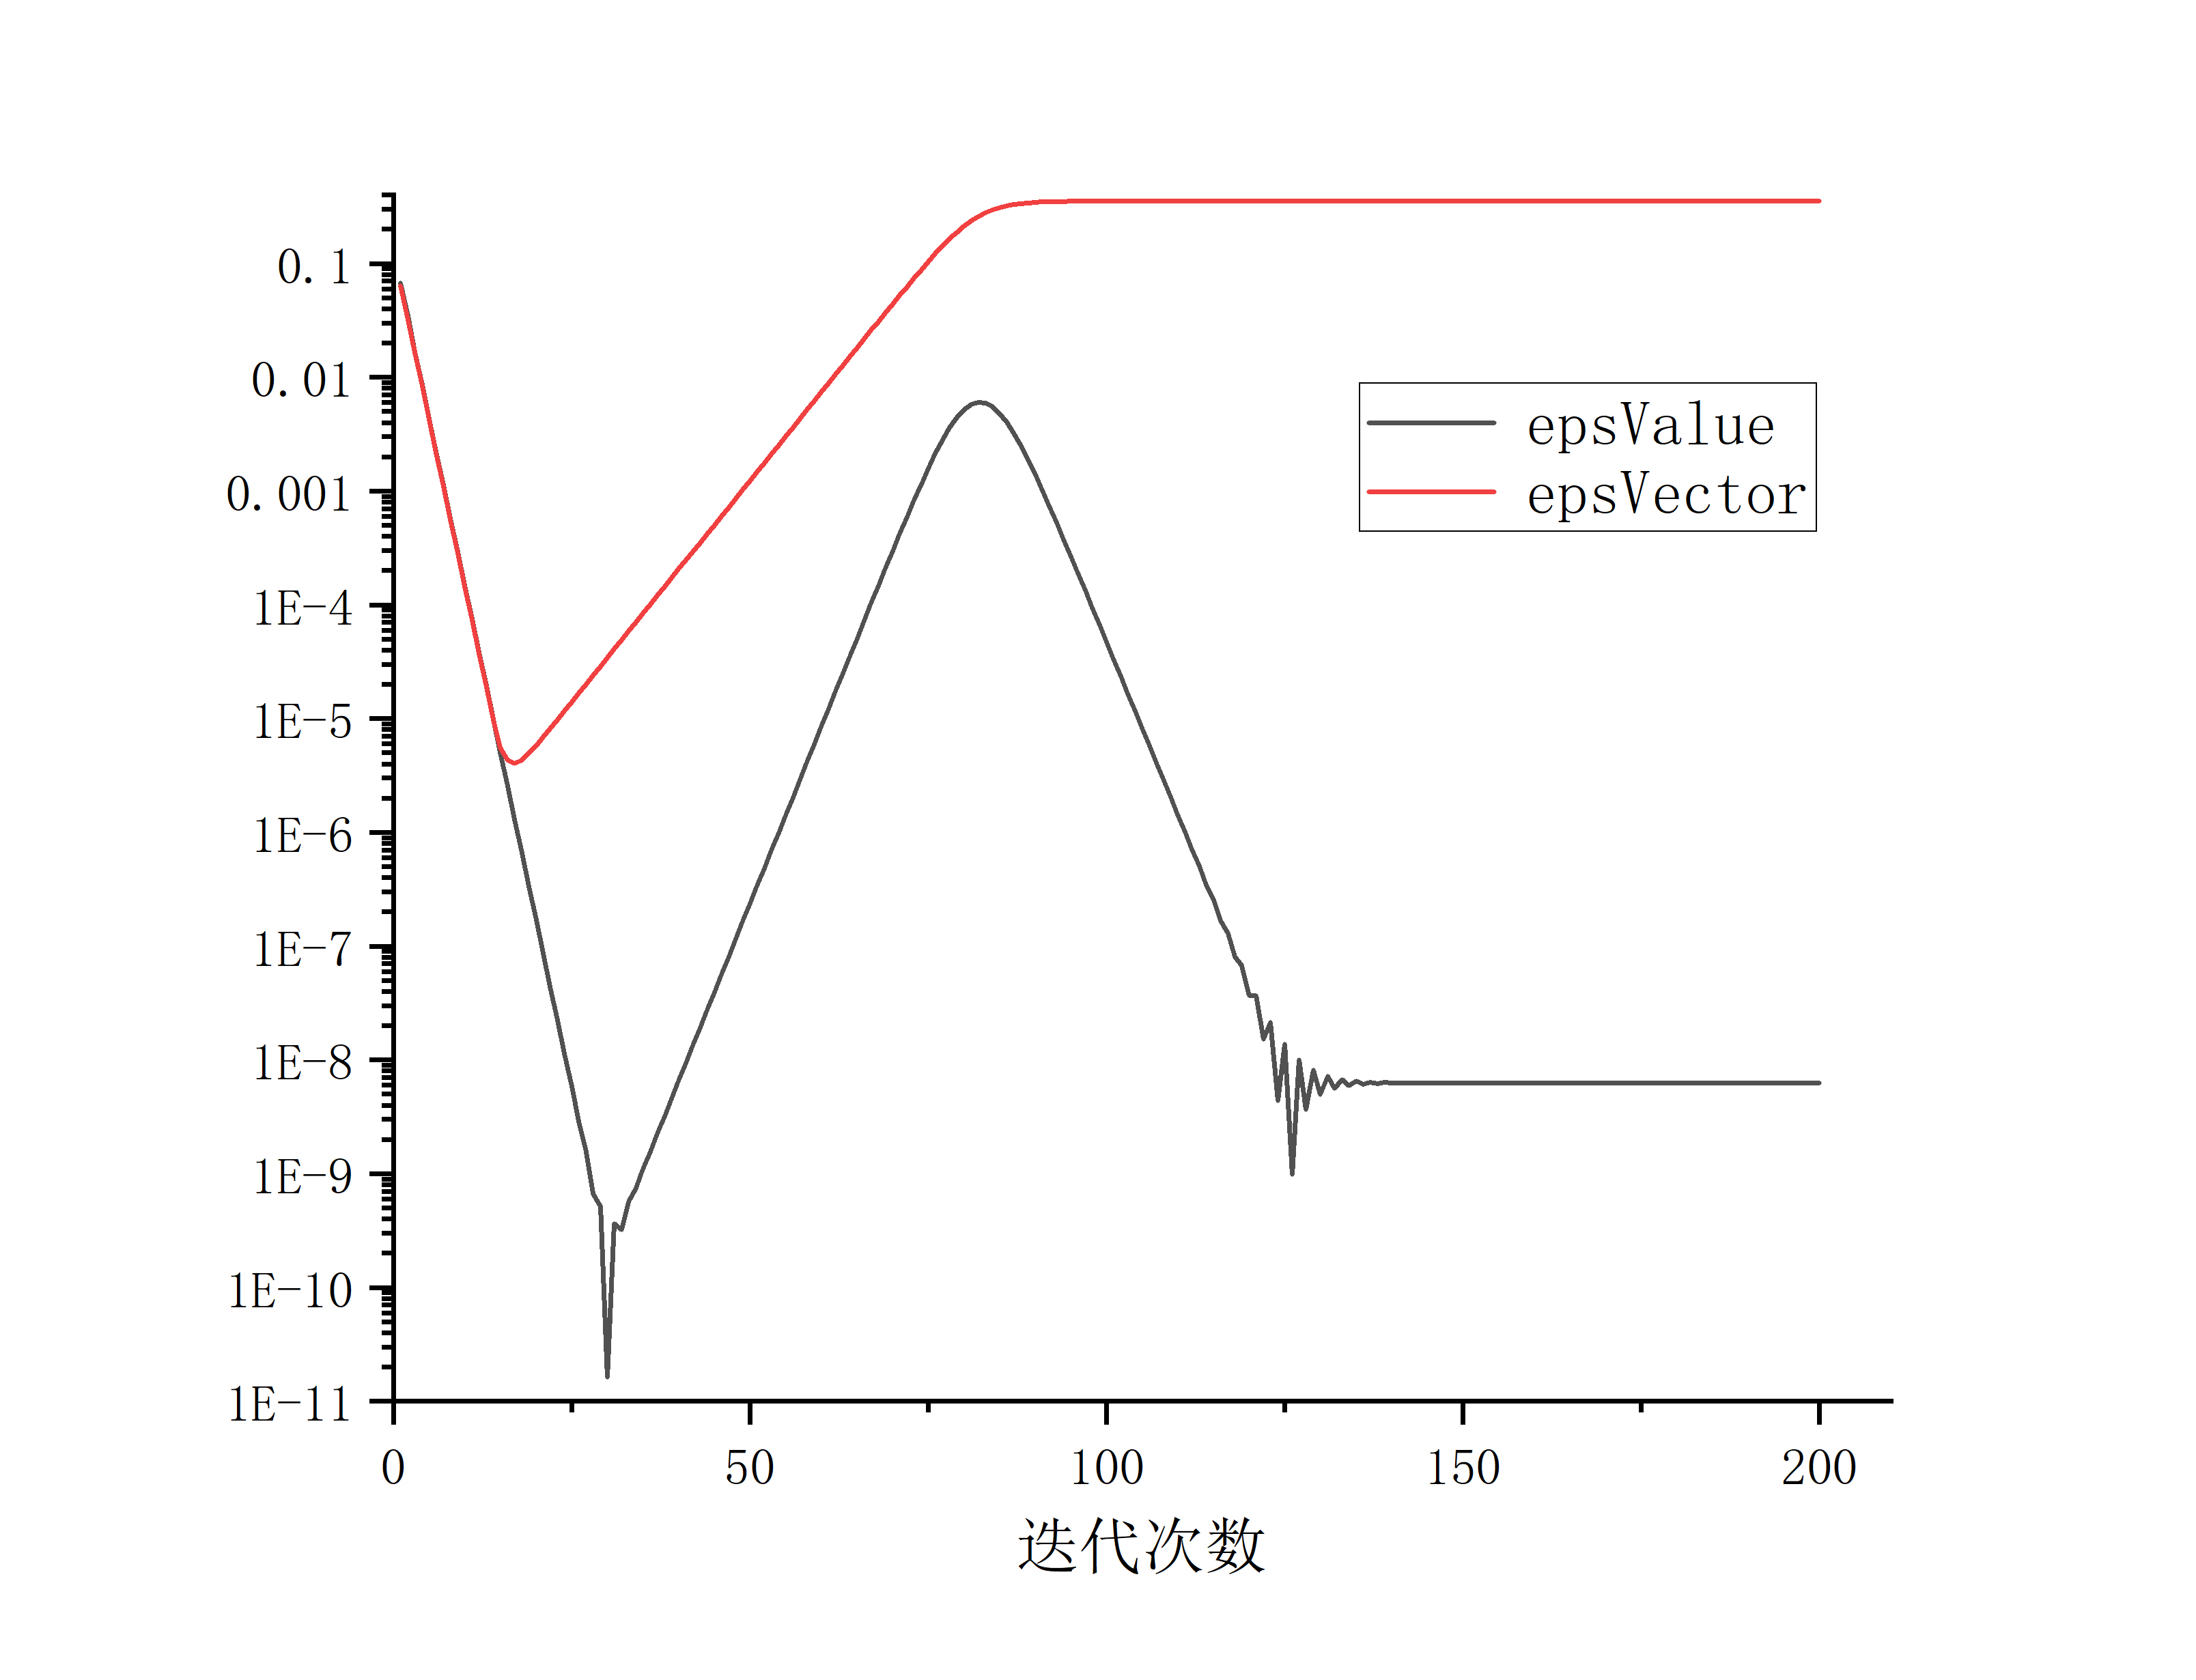
\includegraphics[width=0.8\textwidth]{G=-2迭代过程示意图.jpg}
      \caption{G=-2迭代过程示意图}\label{fig:G=-2迭代过程示意图}
    \end{figure}

    其中epsValue=|相邻两次本征值之差/后一次本征值|,epsVector=相邻两次本征矢之差的无穷范数。如果迭代是收敛的,那么这两个值都应趋于0才对,但实际G=-2时却如上图所示,二者都先变小,后变大,最后保持在一个正常数不变。此时很难说用SCF方法仍然得到了一个收敛的解。之所以第五问得到了收敛的解,其实并没有真的收敛,只是因为判断收敛的条件中收敛精度取$10^{-5}$比较巧的使程序在迭代初期epsValue和epsVector下降到谷底附近时让程序停止了。

    试验得知,当G接近-2时,迭代最终会稳定地在两个态上跳动,即:

    \begin{align*}
      (-\frac{1}{2}\frac{d^2}{dx^2}+V(x)-{(n-1)}g|\phi_1|^2)\phi_2=\epsilon_2 \phi_2\\
      (-\frac{1}{2}\frac{d^2}{dx^2}+V(x)-{(n-1)}g|\phi_2|^2)\phi_1=\epsilon_1 \phi_1
    \end{align*}

    显然,$\phi_1,\phi_2$或他们任意线性组合都不是自洽方程的解,因而用SCF方法不能给出准确的答案。想到第五问所求的特征值(图\ref{fig:q5本征值随G变化示意图}),可能有些是向上面一样的伪收敛。

    于是我们提高精度,再算一遍,收敛精度设为$10^{-7}$,我们认为,如果epsValue和epsVector同时小于这个精度了,那么认为这是良性收敛的,就打出这个特征值;如果在epsValue和epsVector始终不能小于这个精度,而是稳定在某个值不动了,那么认为这是伪收敛,就打出两个反复横跳的特征值。

    代码实现见"../code/q5_ValueCmp.c",输出见"../data/extra/q5_values_cmp.txt"。在txt文本中可以看到,G=-1.8、-1.9、-2.0时程序都输出了两个结果,说明此时是伪收敛,而G从0至-1.7都是真收敛。将特征值和G的关系画出来,并和第五问图\ref{fig:q5本征值随G变化示意图}对比得到

    \begin{figure}[H]
      \centering
      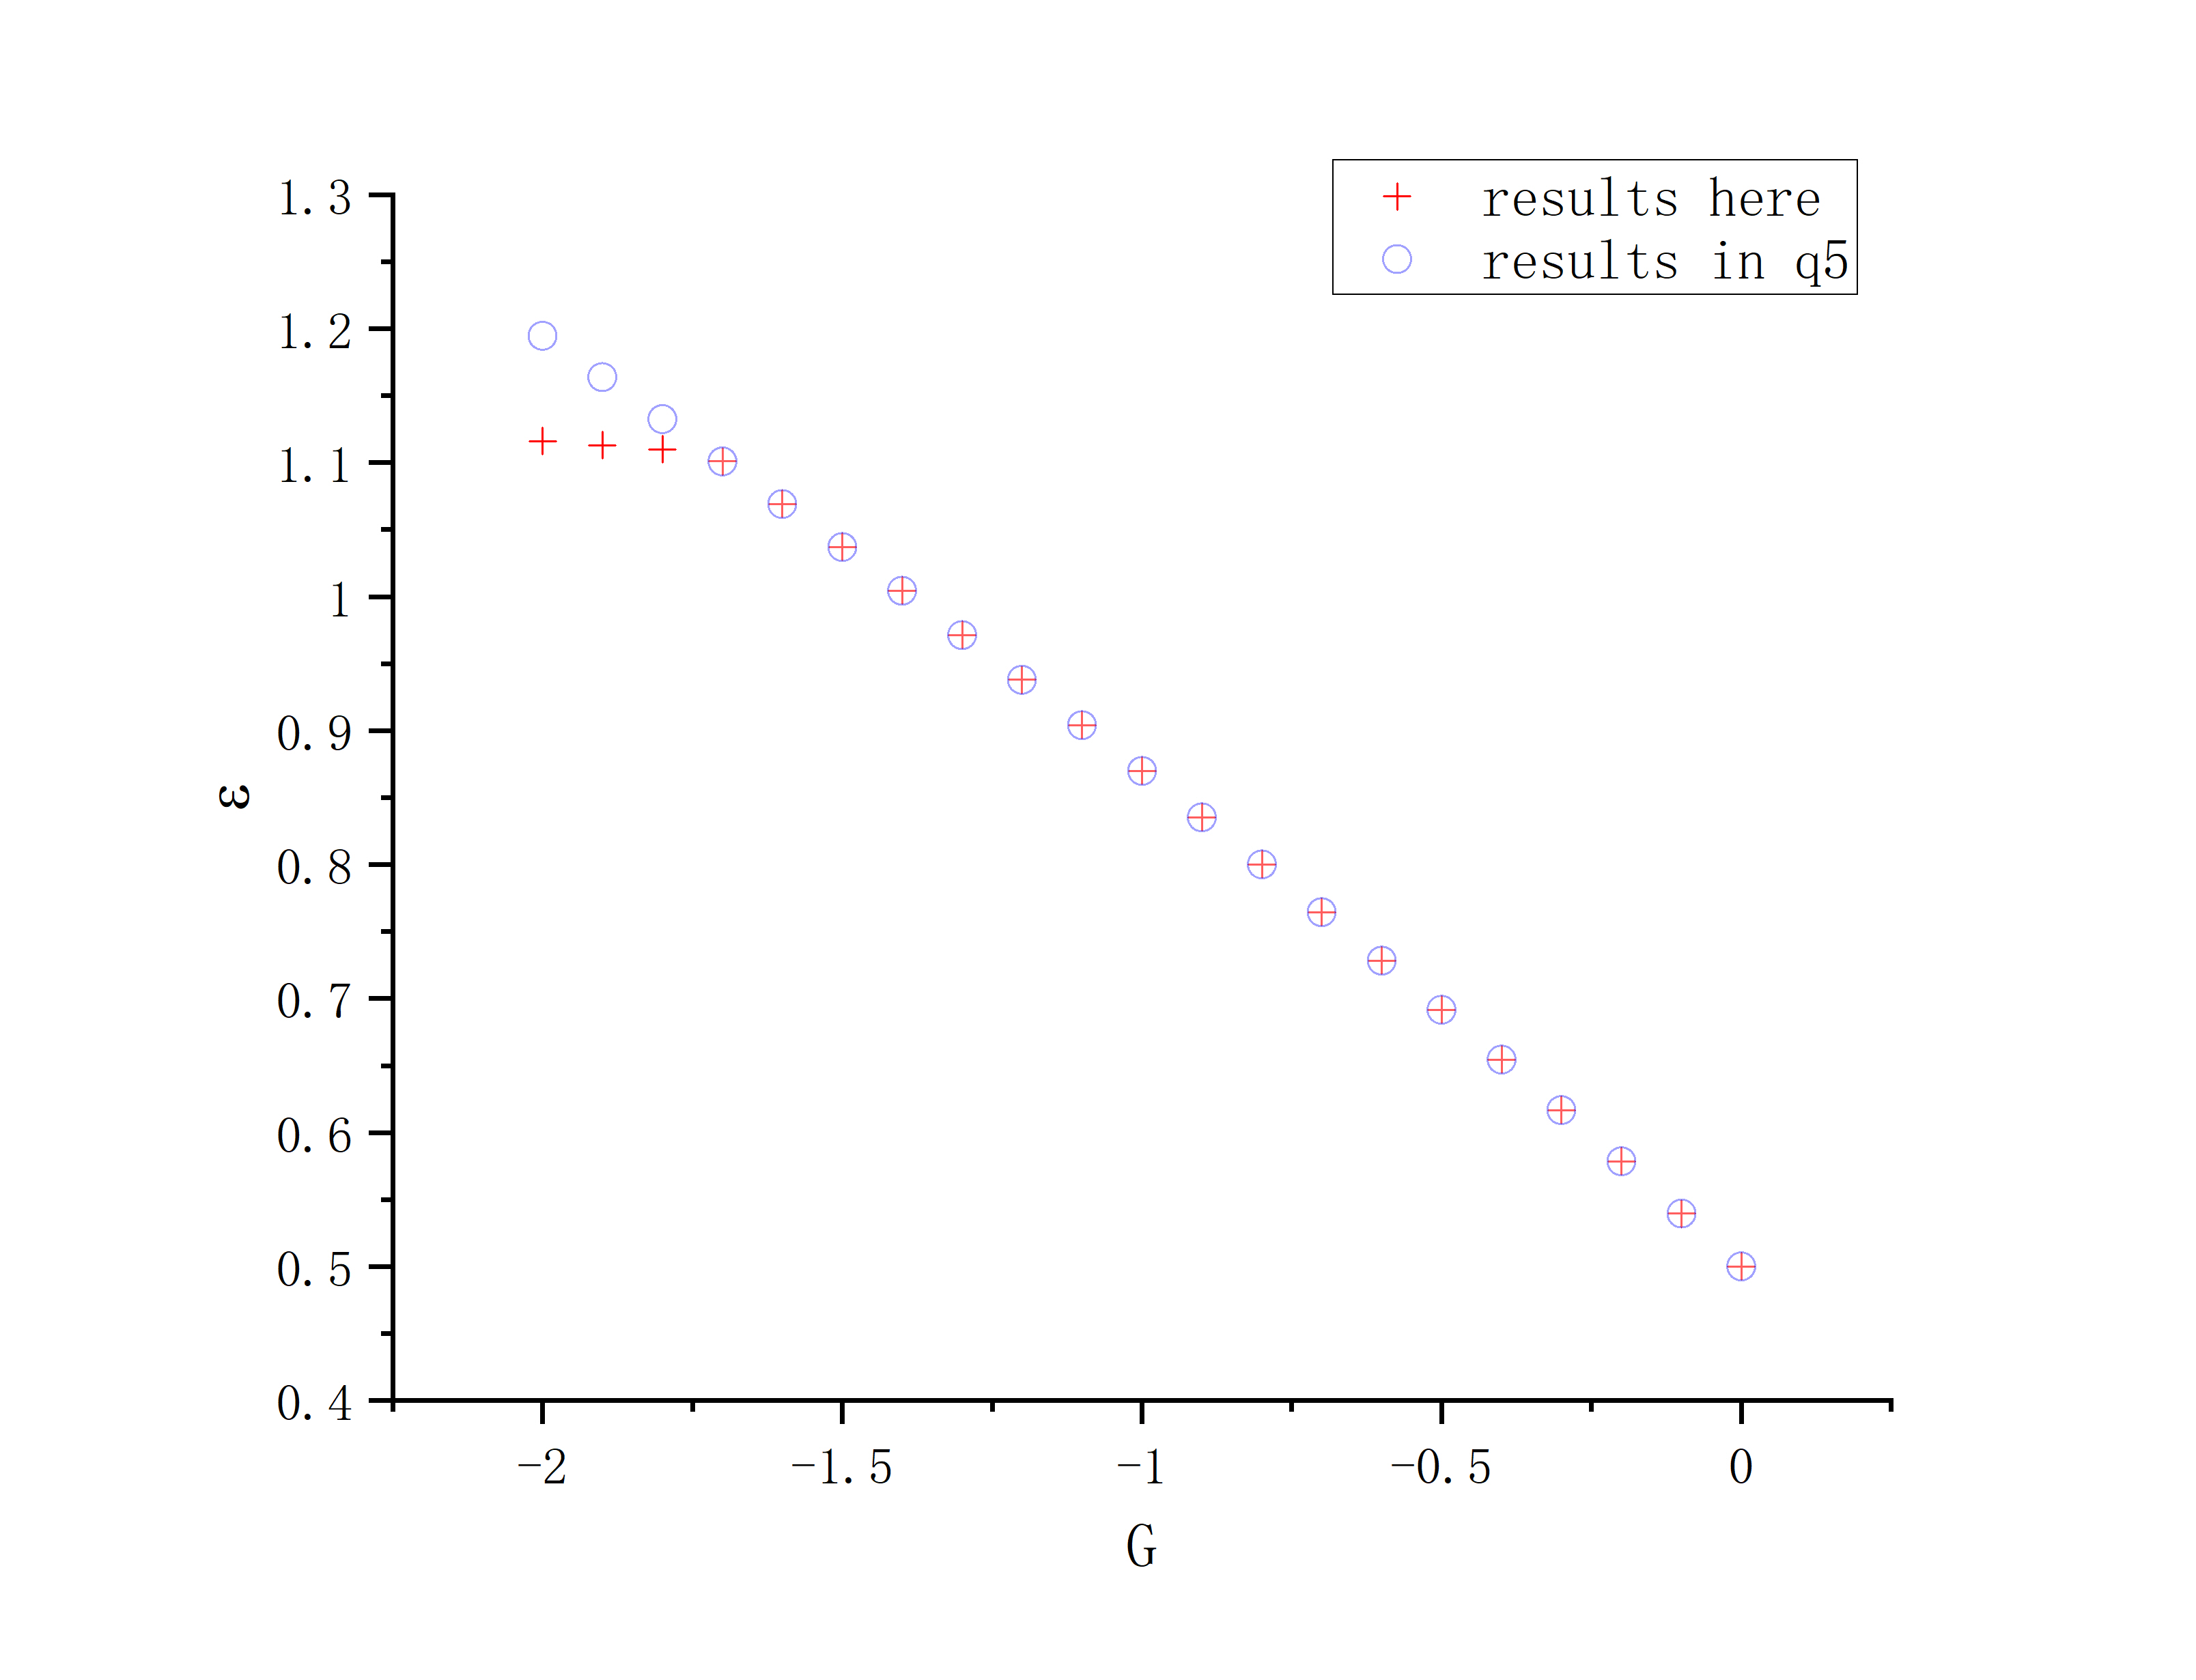
\includegraphics[width=0.8\textwidth]{提升精度后特征值运行结果与第五问对比图.jpg}
      \caption{提升精度后特征值运行结果与第五问对比图}\label{fig:提升精度后特征值运行结果与第五问对比图}
    \end{figure}

    可以看出:

    1. 提升精度后,真收敛的特征值几乎没有变化,说明G从0至-1.7范围内计算的特征值已经收敛;

    2. 伪收敛部分得到的两个横跳的"特征值"近似相等;

    3. 伪收敛部分得到的"特征值"要小于第五问计算结果。

    为探究为何迭代反复横跳后得到的"特征值"更小,我们将G=-1.8,-1.9,-2.0时两个横跳波函数计算出来,并用G=-1.7没有横跳的结果做对比,得到下图
    \footnote{计算程序见"../code/cmpVector.c",数值结果见"../data/extra/cmpVector_G=X.txt"(X=-1.7,-1.8,-1.9,-2.0)}

    \begin{figure}[H]
      \centering
      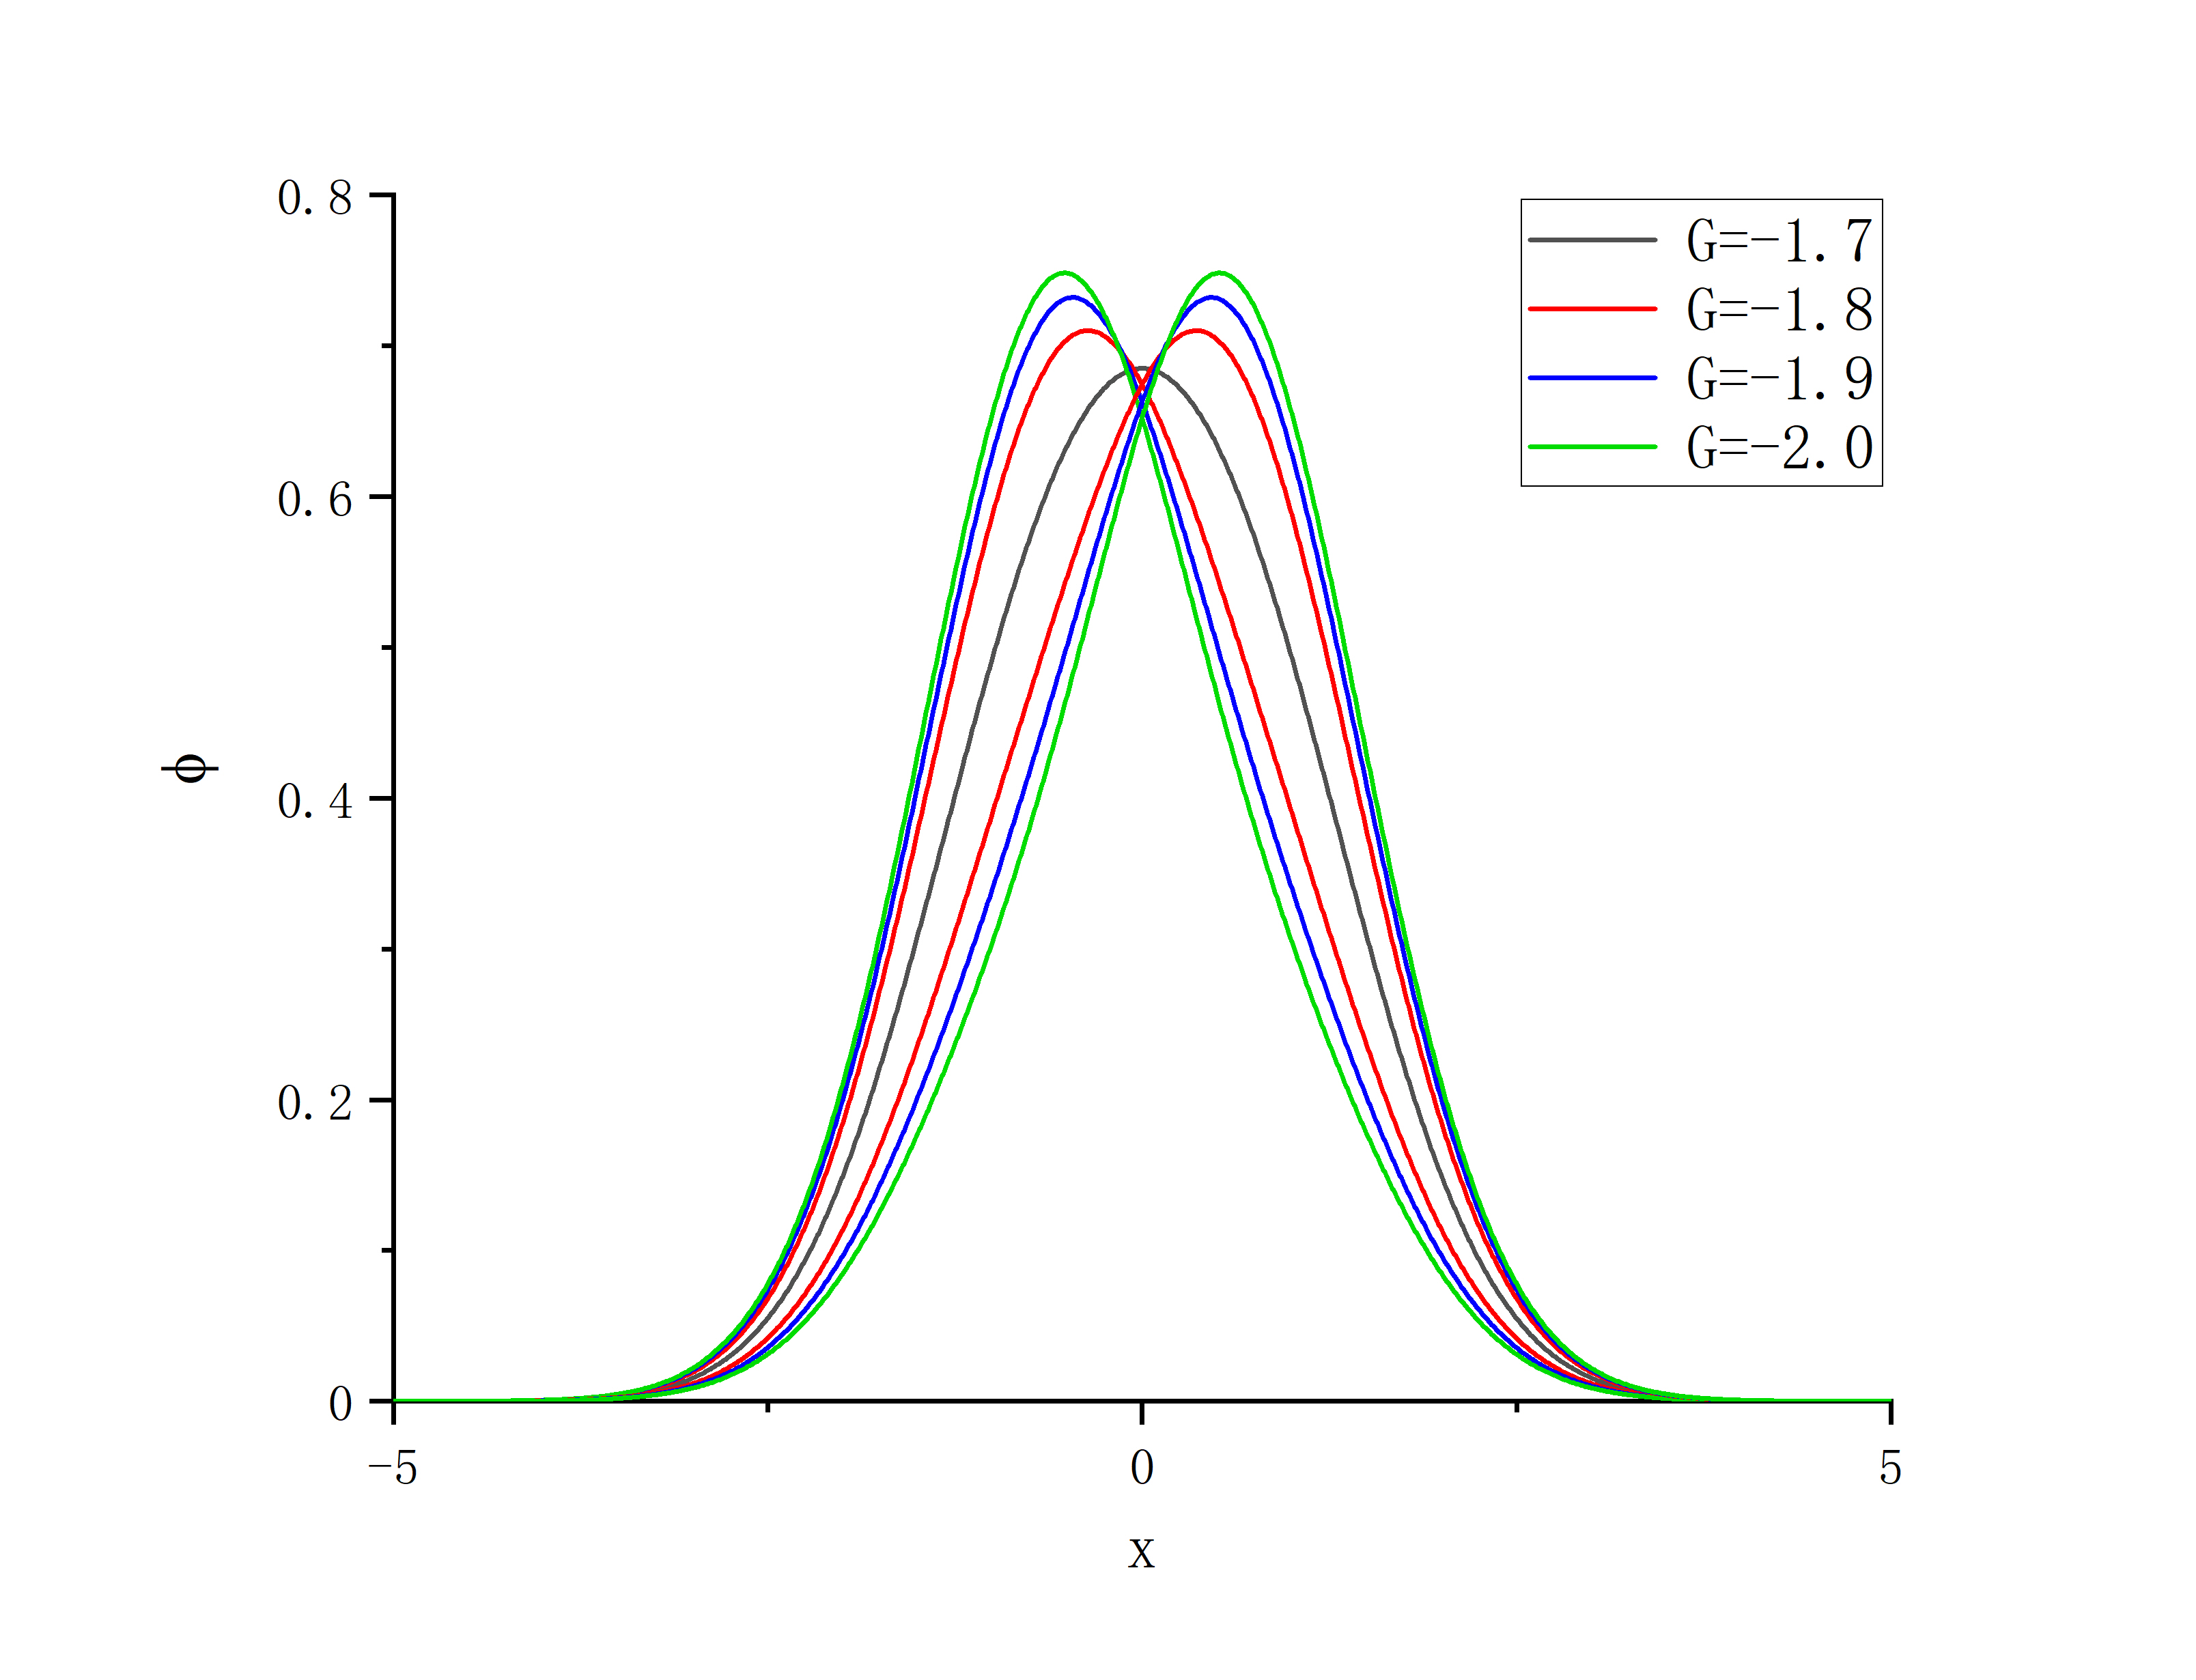
\includegraphics[width=0.8\textwidth]{反复横跳波函数示意图.jpg}
      \caption{反复横跳波函数示意图}\label{fig:反复横跳波函数示意图}
    \end{figure}

    可以看出,G=-1.7仍然收敛到关于原点对称的波函数上,但G=-1.8,-1.9,-2.0均得到两个关于原点对称的波函数,这与第五问的计算结果不同。并且发现,随着|G|的增大,横跳波函数的峰更加远离原点。由于体系关于原点的对称性,我们可以认为这两个波函数是等价的(这可以由两个横跳"特征值"近似相等得到印证),都表示粒子基态的最概然位置偏离原点,并且随着|G|的增大,偏离原点越多。进一步地,考虑到横跳波函数基态能量小于不横跳地波函数基态能量(图\ref{fig:q5精确解和近似解对比图}),说明此时粒子最概然位置偏离原点可以得到一个能量更低的态。这可能是因为,当|G|比较大时,粒子间排斥势十分显著,粒子不倾向于向原点聚拢,而是远离原点,因为在远离原点的地方有一个能量更低的位置,所以波函数峰值偏离原点;而当|G|没有那么大时(|G|<1.7),排斥势不够显著,谐振子势占据主导,粒子都聚集在原点位置,所以波函数峰值在原点。
    
    \begin{thebibliography}{99}  
      \bibitem{ref1}李庆扬,王能超,易大义:数值分析,253页,清华大学出版社,2008年12月第五版
      \bibitem{ref2}李庆扬,王能超,易大义:数值分析,159-160页,清华大学出版社,2008年12月第五版
    \end{thebibliography}
\end{document}